% =====================================================================
%  O Método rDG(P0P1) com HLLC e Minmod — Tutorial Didático (versão ampliada)
%  Compilar com pdflatex (duas vezes). Figuras: scripts/make_figs.sh
% =====================================================================
\documentclass[10pt,a4paper]{article}
\usepackage[utf8]{inputenc}
\usepackage[T1]{fontenc}
\usepackage[brazil]{babel}
\usepackage[margin=2.5cm]{geometry}
\usepackage{amsmath,amssymb,bm}
\usepackage{graphicx}
\usepackage{xcolor}
\usepackage{booktabs}
\usepackage{enumitem}
\usepackage{titlesec}
\usepackage{fancyhdr}
\usepackage[most]{tcolorbox}
\usepackage{listings}
\usepackage{caption}
\usepackage{hyperref}

% ---------------------------------------------------------------- cores
\definecolor{azul}{HTML}{1A5276}
\definecolor{azulclaro}{HTML}{2471A3}
\definecolor{verde}{HTML}{27AE60}
\definecolor{verdeclaro}{HTML}{D5F5E3}
\definecolor{vermelho}{HTML}{E74C3C}
\definecolor{vermelhoclaro}{HTML}{FADBD8}
\definecolor{laranja}{HTML}{E67E22}
\definecolor{amareloclaro}{HTML}{FCF3CF}
\definecolor{cinzacodigo}{HTML}{F4F6F9}
\definecolor{cinzatexto}{HTML}{7F8C8D}

% ---------------------------------------------------------------- títulos
\titleformat{\section}{\Large\bfseries\color{azul}}{\thesection.}{0.6em}{}[{\color{azul}\titlerule}]
\titleformat{\subsection}{\large\bfseries\color{azulclaro}}{\thesubsection}{0.6em}{}
\titlespacing*{\section}{0pt}{18pt}{8pt}
\titlespacing*{\subsection}{0pt}{12pt}{5pt}

% ---------------------------------------------------------------- cabeçalho
\pagestyle{fancy}
\fancyhf{}
\fancyhead[L]{\small\color{cinzatexto}rDG(P0P1) + HLLC + Minmod}
\fancyhead[R]{\small\color{cinzatexto}Tutorial Didático}
\fancyfoot[C]{\thepage}
\renewcommand{\headrulewidth}{0.4pt}
\renewcommand{\headrule}{{\color{cinzatexto}\hrule width\headwidth height\headrulewidth}}

% ---------------------------------------------------------------- caixas
\newtcolorbox{intuicao}{enhanced,colback=verdeclaro,colframe=verde,coltitle=white,colbacktitle=verde,
  fonttitle=\bfseries,title={Intuição},boxrule=0.8pt,arc=2pt,left=6pt,right=6pt,top=5pt,bottom=5pt,
  toptitle=2pt,bottomtitle=2pt,before skip=8pt,after skip=10pt}
\newtcolorbox{atencao}{enhanced,colback=vermelhoclaro,colframe=vermelho,coltitle=white,colbacktitle=vermelho,
  fonttitle=\bfseries,title={Atenção},boxrule=0.8pt,arc=2pt,left=6pt,right=6pt,top=5pt,bottom=5pt,
  toptitle=2pt,bottomtitle=2pt,before skip=8pt,after skip=10pt}
\newtcolorbox{destaque}{enhanced,colback=amareloclaro,colframe=laranja,boxrule=1pt,arc=3pt,
  left=6pt,right=6pt,top=2pt,bottom=2pt,before skip=8pt,after skip=10pt}

% ---------------------------------------------------------------- listagens
\lstset{language=Python,basicstyle=\ttfamily\small,backgroundcolor=\color{cinzacodigo},
  keywordstyle=\color{azulclaro},commentstyle=\color{cinzatexto}\itshape,stringstyle=\color{verde},
  numbers=left,numberstyle=\tiny\color{cinzatexto},numbersep=8pt,frame=single,rulecolor=\color{black!15},
  framerule=0.4pt,xleftmargin=2em,breaklines=true,showstringspaces=false,columns=fullflexible,
  keepspaces=true,inputencoding=utf8,extendedchars=true,
  literate={á}{{\'a}}1 {ã}{{\~a}}1 {â}{{\^a}}1 {é}{{\'e}}1 {ê}{{\^e}}1 {í}{{\'i}}1 {ó}{{\'o}}1 {õ}{{\~o}}1 {ú}{{\'u}}1 {ç}{{\c{c}}}1}
\renewcommand{\lstlistingname}{Listing}
\captionsetup{font=small}

\newcommand{\pd}[2]{\frac{\partial #1}{\partial #2}}
\newcommand{\fh}{\hat f}
\newcommand{\ub}{\bar u}
\newcommand{\uh}{\hat u}
\newcommand{\vu}{\mathbf{u}}
\newcommand{\vf}{\mathbf{f}}

\begin{document}

% ================================================================ capa
\begin{titlepage}
\centering
\vspace*{4.5cm}
{\Huge\bfseries\color{azul} O Método rDG(P0P1)\\[0.4cm] com HLLC e Minmod\par}
\vspace{1.2cm}
{\Large\color{azulclaro} Um Tutorial Didático para o Caso 1D\par}
\vspace{2.2cm}
{\large Leis de conservação hiperbólicas,\\ volumes finitos, Galerkin Descontínuo reconstruído,\\ e o fluxo numérico HLLC\par}
\vspace{2.8cm}
\rule{\textwidth}{0.4pt}\\[0.5cm]
\parbox{0.92\textwidth}{\centering Este documento apresenta, passo a passo, o método rDG(P0P1) aplicado às equações de Euler 1D. Cada conceito é motivado intuitivamente, formalizado com equações e ilustrado com código Python e gráficos. Esta versão ampliada detalha as deduções, acrescenta exemplos numéricos resolvidos à mão, um estudo de convergência e figuras novas, geradas por uma implementação de referência que acompanha o texto.}
\vfill
\end{titlepage}

\setcounter{page}{1}
\tableofcontents
\newpage

% ================================================================ 1
\section{Leis de conservação e o conceito de fluxo}

\subsection{O que estamos resolvendo?}

Imagine uma quantidade física --- por exemplo, a massa de um gás --- distribuída ao longo de um tubo unidimensional. Essa quantidade pode se mover (ser \emph{transportada}) ao longo do tubo, mas não pode ser criada nem destruída. Isso é uma \textbf{lei de conservação}:
\begin{destaque}
\begin{equation}\label{eq:lei}
\pd{u}{t}+\pd{f(u)}{x}=0
\end{equation}
\end{destaque}
Aqui:
\begin{itemize}[leftmargin=2.2em,itemsep=2pt]
\item[] $u(x,t)$ é a \textbf{variável conservativa} (ex.: densidade, momento, energia);
\item[] $f(u)$ é o \textbf{fluxo}: ele mede \emph{quanto de $u$ passa por um ponto $x$ por unidade de tempo}.
\end{itemize}

\begin{intuicao}
Pense em um rio: $u$ é a concentração de um corante na água; $f(u)$ é a ``vazão de corante'' passando por cada seção do rio. Se entra mais corante do que sai de um trecho, a concentração naquele trecho aumenta --- é exatamente isso que a equação \eqref{eq:lei} diz.
\end{intuicao}

Vale a pena ver essa frase escrita em fórmula, porque é dela que nasce o método numérico. Integre \eqref{eq:lei} num trecho fixo $[a,b]$ do tubo. O primeiro termo dá a taxa de variação do total de $u$ no trecho; o segundo é a integral de uma derivada, que vale a diferença do fluxo nas pontas:
\begin{equation}\label{eq:balanco}
\frac{d}{dt}\int_a^b u(x,t)\,dx=f\big(u(a,t)\big)-f\big(u(b,t)\big).
\end{equation}
Esta é a \textbf{forma integral} da lei de conservação: ``o que há dentro só muda pelo que atravessa as fronteiras''. Ela tem uma vantagem decisiva sobre \eqref{eq:lei}: não pede que $u$ seja derivável. Quando a solução desenvolve um salto (um choque), a forma diferencial perde o sentido, mas a forma integral continua válida. É por isso que os métodos de volumes finitos partem de \eqref{eq:balanco}, não de \eqref{eq:lei}.

Uma última observação sobre \eqref{eq:lei}. Pela regra da cadeia, $\partial_x f(u)=f'(u)\,\partial_xu$, de modo que a equação pode ser lida como $\partial_tu+f'(u)\,\partial_xu=0$: a informação é transportada com a \textbf{velocidade característica} $f'(u)$. Essa velocidade decide tudo o que vem depois: para onde a informação viaja, qual lado da interface ``manda'' e qual passo de tempo um método explícito poderia usar.

\subsection{Exemplo fundamental: a equação de Burgers}

O exemplo mais simples e instrutivo de lei de conservação não-linear é a \textbf{equação de Burgers inviscida}:
\begin{equation}\label{eq:burgers}
\pd{u}{t}+\pd{}{x}\left(\frac{u^2}{2}\right)=0
\end{equation}
Aqui o fluxo é $f(u)=\tfrac12u^2$; a ``velocidade de propagação'' é $f'(u)=u$: quanto maior o valor de $u$, mais rápido ele se propaga. Essa não-linearidade faz com que perfis suaves possam \emph{quebrar} e formar \textbf{choques} (descontinuidades) em tempo finito --- um dos grandes desafios que todo método numérico precisa enfrentar.

\begin{intuicao}
Imagine carros numa estrada em que cada carro anda com velocidade igual ao seu ``valor de $u$''. Os carros rápidos, atrás, alcançam os lentos, na frente; a fila se comprime até virar uma parede: o choque. Para um perfil inicial $u_0(x)$, isso acontece no instante $t_b=-1/\min u_0'(x)$, o momento em que duas características se cruzam pela primeira vez. Depois de $t_b$ a solução suave deixa de existir; só a forma integral \eqref{eq:balanco} dá sentido ao que acontece; ela fixa a velocidade do choque em $s=\tfrac12(u_L+u_R)$, a média dos valores dos dois lados.
\end{intuicao}

\subsection{Sistema: as equações de Euler 1D}

Para a dinâmica de gases, a lei de conservação é um \textbf{sistema} com três componentes:
\begin{destaque}
\begin{equation}\label{eq:euler}
\vu=\begin{pmatrix}\rho\\ \rho v\\ E\end{pmatrix},\qquad
\vf(\vu)=\begin{pmatrix}\rho v\\ \rho v^2+p\\ (E+p)\,v\end{pmatrix}
\end{equation}
\end{destaque}
com a equação de estado do gás ideal:
\begin{equation}\label{eq:eos}
p=(\gamma-1)\big(E-\tfrac12\rho v^2\big)
\end{equation}
Cada linha é uma conservação: de massa ($\rho$), de momento ($\rho v$) e de energia ($E$). O fluxo agora é um vetor que acopla as três quantidades.

Lendo as componentes do fluxo linha a linha fica claro de onde vem cada uma: a massa é transportada com velocidade $v$ (fluxo $\rho v$); o momento é transportado ($\rho v\cdot v$) e, além disso, empurrado pela pressão ($p$); a energia é transportada ($Ev$) e a pressão realiza trabalho ($pv$). A variável $E$ é a energia total por unidade de volume: energia interna $\rho e$ mais energia cinética $\tfrac12\rho v^2$. Para o gás ideal, $p=(\gamma-1)\rho e$, o que dá \eqref{eq:eos}; usaremos $\gamma=1{,}4$ (ar).

\begin{intuicao}
O sistema de Euler é a ``versão séria'' de Burgers: em vez de uma única velocidade escalar, temos três tipos de ondas --- duas ondas acústicas (se propagando a $v\pm a$, onde $a=\sqrt{\gamma p/\rho}$ é a velocidade do som) e uma onda de contato (se propagando a $v$). É para resolver essas três ondas corretamente que usaremos o fluxo HLLC.

As três velocidades são os autovalores da matriz jacobiana $\partial\vf/\partial\vu$; o fato de serem reais e distintas é o que torna o sistema \emph{hiperbólico} e garante que a informação viaja com velocidade finita. A onda de contato é especial: através dela a pressão e a velocidade são contínuas e só a densidade salta, como a fronteira entre dois gases de temperaturas diferentes que se movem juntos. Nenhum mecanismo a comprime, por isso ela é a onda mais difícil de manter nítida numericamente.
\end{intuicao}

% ================================================================ 2
\section{Discretização: de contínuo para discreto}

\subsection{A malha}

Dividimos o domínio em $N$ células:
\[
I_i=[x_{i-1/2},\,x_{i+1/2}],\qquad i=0,1,\dots,N-1
\]
com centro $x_i$ e tamanho $\Delta x=x_{i+1/2}-x_{i-1/2}$.

Os pontos $x_{i\pm1/2}$ são as \textbf{interfaces} (ou faces) entre células vizinhas; é nelas que toda a comunicação acontece. Para tratar os contornos sem casos especiais, acrescentamos uma \textbf{célula fantasma} em cada extremidade e copiamos nela o valor da célula vizinha. Isso implementa a condição \emph{transmissiva}: as ondas saem do domínio como se o tubo continuasse. Para um domínio periódico, a célula fantasma recebe o valor da célula do outro extremo.

\subsection{A média celular e a forma integral}

A ideia-chave dos volumes finitos é trabalhar com a \textbf{média celular}:
\begin{destaque}
\begin{equation}\label{eq:media}
\ub_i(t)=\frac{1}{\Delta x}\int_{x_{i-1/2}}^{x_{i+1/2}}u(x,t)\,dx
\end{equation}
\end{destaque}

Se integrarmos a lei de conservação \eqref{eq:lei} sobre a célula $I_i$, obtemos:
\begin{equation}\label{eq:fv}
\frac{d\ub_i}{dt}=-\frac{1}{\Delta x}\Big[\fh_{i+1/2}-\fh_{i-1/2}\Big]
\end{equation}
onde $\fh_{i+1/2}$ é o \textbf{fluxo numérico} na interface entre as células $i$ e $i+1$.

Vale percorrer o caminho de \eqref{eq:lei} até \eqref{eq:fv} com calma, porque ele mostra onde entra a única aproximação do método. Aplique a forma integral \eqref{eq:balanco} ao trecho $[a,b]=[x_{i-1/2},x_{i+1/2}]$ e divida por $\Delta x$:
\[
\frac{d\ub_i}{dt}=-\frac{1}{\Delta x}\Big[f\big(u(x_{i+1/2},t)\big)-f\big(u(x_{i-1/2},t)\big)\Big].
\]
Até aqui \emph{nada} foi aproximado: esta relação é exata para a solução verdadeira. O problema é que o método só conhece as médias $\ub_i$, não os valores pontuais $u(x_{i\pm1/2},t)$ nas interfaces. A aproximação consiste em substituir o fluxo físico na interface por um \emph{fluxo numérico} $\fh_{i+1/2}$, calculado a partir das médias das células vizinhas. Como escolher esse fluxo é o assunto dos Passos 1 a 3.

\begin{intuicao}
A equação \eqref{eq:fv} é um \textbf{balanço de caixa}: a taxa de variação da média $\ub_i$ é igual ao fluxo que entra pela esquerda ($\fh_{i-1/2}$) menos o fluxo que sai pela direita ($\fh_{i+1/2}$), dividido pelo tamanho da célula. Se entra mais do que sai, $\ub_i$ aumenta; se sai mais, diminui. É exatamente isso que a Figura~\ref{fig:tempo} ilustra.

Há uma consequência imediata e preciosa: o fluxo que sai da célula $i$ pela face $x_{i+1/2}$ é o mesmo que entra na célula $i+1$. Somando \eqref{eq:fv} sobre todas as células, os fluxos interiores cancelam aos pares e o total $\sum_i\ub_i\Delta x$ só muda pelo que atravessa as duas extremidades do domínio. O método é \textbf{conservativo por construção}, com ou sem choques; é isso que garante que os choques numéricos andem na velocidade certa.
\end{intuicao}

\begin{figure}[htbp]
\centering
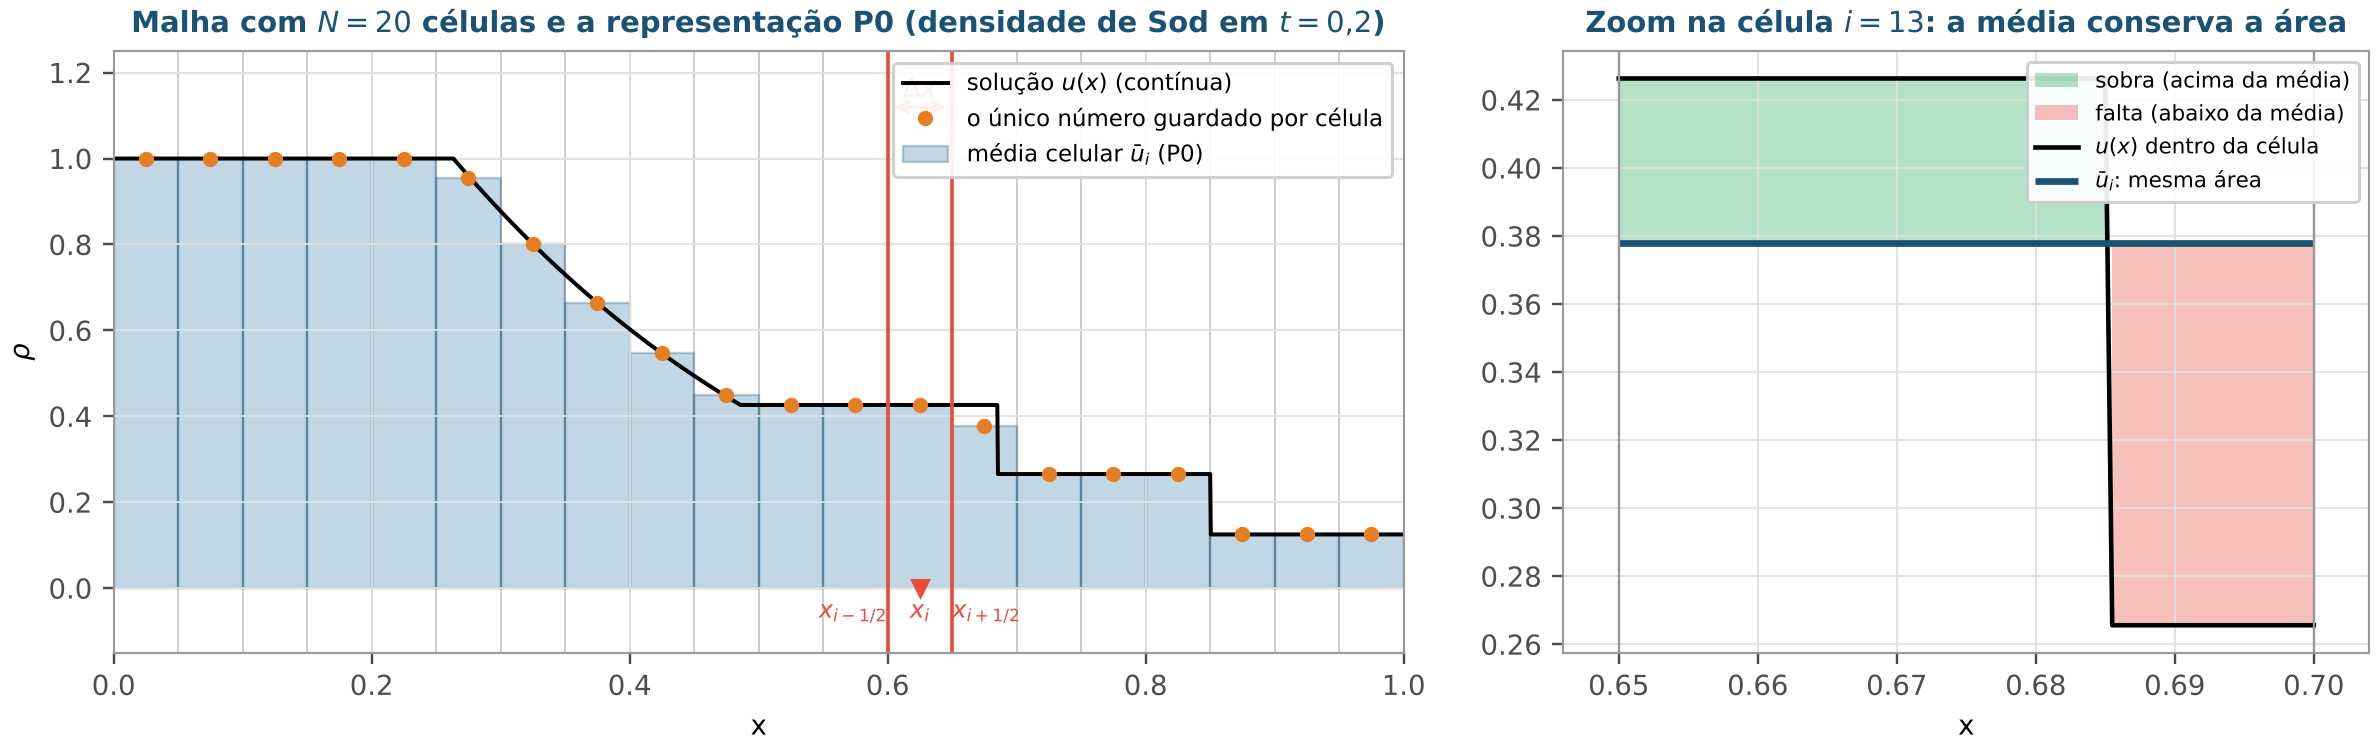
\includegraphics[width=\textwidth]{figs/fig1_malha.png}
\caption{A malha e as médias celulares $\ub_i$. Como exemplo usamos a densidade da solução exata do tubo de choque de Sod em $t=0{,}2$ (curva preta), que tem uma parte suave e dois saltos. Esquerda: cada célula armazena um único número, a média da solução naquela célula --- esta é a representação P0 (constante por partes). Note o que se perde: a rampa suave vira uma escada e os saltos ficam ``escondidos'' dentro de uma célula. Direita: zoom numa célula que contém o salto; a média é a altura do retângulo que tem a mesma área que a curva, a parte verde (sobra) compensa a vermelha (falta).}
\label{fig:malha}
\end{figure}

% ================================================================ 3
\section{De volumes finitos a Galerkin Descontínuo (e por que ``reconstruído'')}

\subsection{O problema de primeira ordem}

O método de volumes finitos descrito acima --- com médias constantes por célula --- é de \textbf{primeira ordem} de precisão. Isso significa que o erro diminui linearmente com $\Delta x$: para cortar o erro pela metade, precisamos dobrar o número de células. Na prática, isso gera soluções muito difusas, com choques ``borrados'' e regiões suaves mal resolvidas.

\begin{intuicao}
De onde vem a primeira ordem? Ao representar a solução por um valor constante em cada célula, cometemos em cada interface um erro proporcional à inclinação local vezes $\Delta x$ (a diferença entre o valor na face e a média). O fluxo numérico transforma esse erro num ``atrito'' numérico: a solução se comporta como se tivesse uma viscosidade artificial proporcional a $\Delta x$. É essa viscosidade que borra os choques e achata os picos. Com uma reta por célula, o erro na face cai para a ordem de $\Delta x^2$ (a curvatura vezes $\Delta x^2$) e a viscosidade artificial desaparece nas regiões suaves.
\end{intuicao}

Para obter \textbf{segunda ordem}, precisamos de mais informação dentro de cada célula. Há dois caminhos clássicos:
\begin{enumerate}[leftmargin=2.5em,itemsep=3pt]
\item \textbf{MUSCL} (Monotone Upstream-centred Schemes for Conservation Laws): mantém apenas as médias $\ub_i$ como incógnitas e \textbf{reconstrói} uma inclinação $\uh_i$ a cada passo usando as médias vizinhas.
\item \textbf{DG (Galerkin Descontínuo)}: armazena e evolui \textbf{ambos} $\ub_i$ e $\uh_i$ como incógnitas independentes, cada uma com sua própria equação de evolução.
\end{enumerate}

\subsection{A formulação DG(P1)}

No DG, a solução dentro de cada célula é um polinômio:
\begin{equation}\label{eq:dg}
u_h(x)\big|_{I_i}=\ub_i\,\varphi_0(\xi)+\uh_i\,\varphi_1(\xi),\qquad \varphi_0=1,\ \ \varphi_1=\xi
\end{equation}
onde $\xi=\frac{x-x_i}{\Delta x/2}\in[-1,+1]$ é a coordenada local. A formulação fraca (multiplicar por funções-teste $\varphi_k$ e integrar) produz \emph{duas} equações por célula:
\begin{equation}\label{eq:fraca}
\int_{I_i}\pd{u_h}{t}\,\varphi_k\,dx-\int_{I_i}f(u_h)\,\frac{d\varphi_k}{dx}\,dx+\Big[\fh\,\varphi_k\Big]_{x_{i-1/2}}^{x_{i+1/2}}=0,\qquad k=0,1
\end{equation}
\begin{itemize}[leftmargin=2.5em,itemsep=3pt]
\item $k=0$ ($\varphi_0=1$): dá a equação de volumes finitos para $\ub_i$ --- é exatamente \eqref{eq:fv};
\item $k=1$ ($\varphi_1=\xi$): dá uma equação \emph{adicional} para evoluir $\uh_i$ no tempo.
\end{itemize}

Dois detalhes da escolha da base merecem atenção. Primeiro, $\varphi_1=\xi$ tem média zero na célula ($\int_{-1}^{1}\xi\,d\xi=0$), logo o coeficiente $\ub_i$ em \eqref{eq:dg} é \emph{sempre} a média celular, qualquer que seja $\uh_i$: a reta passa pela média no centro da célula. Segundo, $\uh_i$ é a variação da reta do centro até a face: nos extremos $\xi=\pm1$ a solução vale $\ub_i\pm\uh_i$. A inclinação física é $2\uh_i/\Delta x$. Guardar esses dois significados em mente evita confusões de fatores $2$ e $\tfrac12$ mais adiante.

Como \eqref{eq:fraca} aparece: multiplica-se \eqref{eq:lei} por $\varphi_k$, integra-se na célula e integra-se por partes o termo de fluxo. A integração por partes transfere a derivada do fluxo para a função-teste (o termo de volume) e deixa nas faces o fluxo avaliado nos contornos (o termo de fronteira). Como $u_h$ é descontínua nas faces, o fluxo ali precisa ser o fluxo numérico $\fh$, o mesmo do método de volumes finitos. Para $k=1$ o termo de volume não é nulo e exige quadratura de Gauss; o termo $\int\partial_tu_h\,\varphi_k\,dx$ gera uma pequena \emph{matriz de massa} por célula.

\subsection{O caminho ``reconstruído'': rDG(P0P1)}

O DG(P1) é elegante, mas tem um custo: precisa evoluir $2N$ incógnitas em vez de $N$; além disso, a integral do fluxo com $\varphi_1$ é não-trivial (envolve quadratura de Gauss).

O \textbf{rDG(P0P1)} (reconstructed DG) é um híbrido:
\begin{destaque}
\begin{itemize}[leftmargin=1.8em,itemsep=3pt]
\item \textbf{Evolui apenas} as médias $\ub_i$ (equação com $k=0$, ou seja, FV puro);
\item \textbf{Reconstrói} a inclinação $\uh_i$ a partir dos vizinhos a cada passo, em vez de evoluir via $k=1$.
\end{itemize}
\end{destaque}

A notação $P_nP_m$ resume a família: guarda-se e evolui-se um polinômio de grau $n$, mas usa-se nos fluxos um polinômio reconstruído de grau $m\ge n$. Assim rDG(P0P0) é o volume finito de primeira ordem, rDG(P0P1) é o método deste tutorial, rDG(P1P2) guarda a reta e reconstrói a parábola (terceira ordem) e DG(P1) é o caso sem reconstrução, $n=m=1$. A reconstrução é possível porque a informação ``que falta'' na célula $i$ está disponível nas células vizinhas; o rDG apenas a recupera no momento do uso, em vez de carregá-la como incógnita.

\begin{intuicao}
O rDG(P0P1) é essencialmente um método MUSCL, mas formulado na linguagem DG. A vantagem dessa formulação é tripla: (i) a extensão para ordens superiores é sistemática (rDG(P0P2), rDG(P1P2), etc.); (ii) a análise de estabilidade e convergência se apoia na teoria DG; (iii) a implementação se integra naturalmente a frameworks DG existentes.
\end{intuicao}

% ================================================================ 4
\section{Passo 1: reconstrução com minmod}

\subsection{A inclinação limitada}

Precisamos calcular $\uh_i$ a partir das médias vizinhas. A maneira mais natural é usar diferenças:
\begin{equation}\label{eq:deltas}
\Delta_{+i}=\ub_{i+1}-\ub_i\quad\text{(forward)},\qquad \Delta_{-i}=\ub_i-\ub_{i-1}\quad\text{(backward)}
\end{equation}
Se ambas concordam em sinal, o perfil é localmente monótono e podemos usar a menor das duas (em valor absoluto) como inclinação. Se discordam, estamos num extremo local ou choque; a inclinação deve ser zero. Isso é o \textbf{limitador minmod}:
\begin{destaque}
\begin{equation}\label{eq:minmod}
\uh_i=\frac12\,\mathrm{minmod}(\Delta_{+i},\Delta_{-i})\equiv\frac12
\begin{cases}
\mathrm{sgn}(\Delta_{+i})\,\min(|\Delta_{+i}|,|\Delta_{-i}|) & \text{se }\Delta_{+i}\cdot\Delta_{-i}>0\\[2pt]
0 & \text{caso contrário}
\end{cases}
\end{equation}
\end{destaque}

De onde vem o fator $\tfrac12$? Se a solução fosse exatamente uma reta, teríamos $\Delta_{+i}=\Delta_{-i}=\Delta$ e a reta subiria $\Delta$ de um centro de célula ao seguinte, ou seja, $\Delta/2$ do centro até a face. Como $\uh_i$ é justamente a variação do centro até a face (Seção~3.2), a escolha $\uh_i=\Delta/2$ reproduz a reta sem erro. Sem o limitador, a opção natural seria a média das duas diferenças, $\uh_i=\tfrac14(\Delta_{+i}+\Delta_{-i})=\tfrac14(\ub_{i+1}-\ub_{i-1})$, a boa e velha diferença central. O minmod troca a média pela menor das duas, em módulo: é a versão ``cautelosa'' da diferença central.

\paragraph{Um exemplo à mão.} Tome três médias consecutivas $\ub_{i-1}=0{,}20$, $\ub_i=0{,}50$ e $\ub_{i+1}=0{,}60$. Então $\Delta_{-i}=0{,}30$ e $\Delta_{+i}=0{,}10$: mesmo sinal, logo $\uh_i=\tfrac12\cdot0{,}10=0{,}05$ e os valores de face são $0{,}45$ e $0{,}55$, ambos dentro do intervalo dos vizinhos. A diferença central daria $\uh_i=0{,}10$ e o valor de face $0{,}60$, igual ao vizinho da direita: uma inclinação no limite do aceitável. Agora troque $\ub_{i+1}$ por $0{,}40$: $\Delta_{+i}=-0{,}10$ discorda de $\Delta_{-i}=+0{,}30$, a célula é um máximo local e $\uh_i=0$.

\begin{intuicao}
\textbf{(a) Quando os dois vizinhos concordam} (mesma direção de variação), o minmod escolhe a inclinação \textbf{mais conservadora} (menor em módulo). Isso evita que a reconstrução crie ``overshoots'' além dos dados: os valores de face ficam sempre entre a média da célula e a média do vizinho correspondente.

\textbf{(b) Quando os vizinhos discordam} (um cresce e outro decresce: extremo local ou choque), ele \textbf{zera a inclinação}. Nesse caso, a célula degenera para P0 (constante); o método cai para primeira ordem \emph{localmente}. Essa degeneração é proposital: é o preço que pagamos para evitar oscilações espúrias (fenômeno de Gibbs) perto de descontinuidades.

O nome técnico dessa propriedade é TVD (\emph{total variation diminishing}): a soma dos saltos $\sum_i|\ub_{i+1}-\ub_i|$ nunca aumenta de um passo para o outro, logo nenhuma oscilação nova pode nascer. Há um teorema de Godunov dizendo que nenhum esquema \emph{linear} consegue ser ao mesmo tempo de segunda ordem e livre de oscilações; o limitador é a saída não linear, porque a inclinação depende dos próprios dados.
\end{intuicao}

\begin{figure}[htbp]
\centering
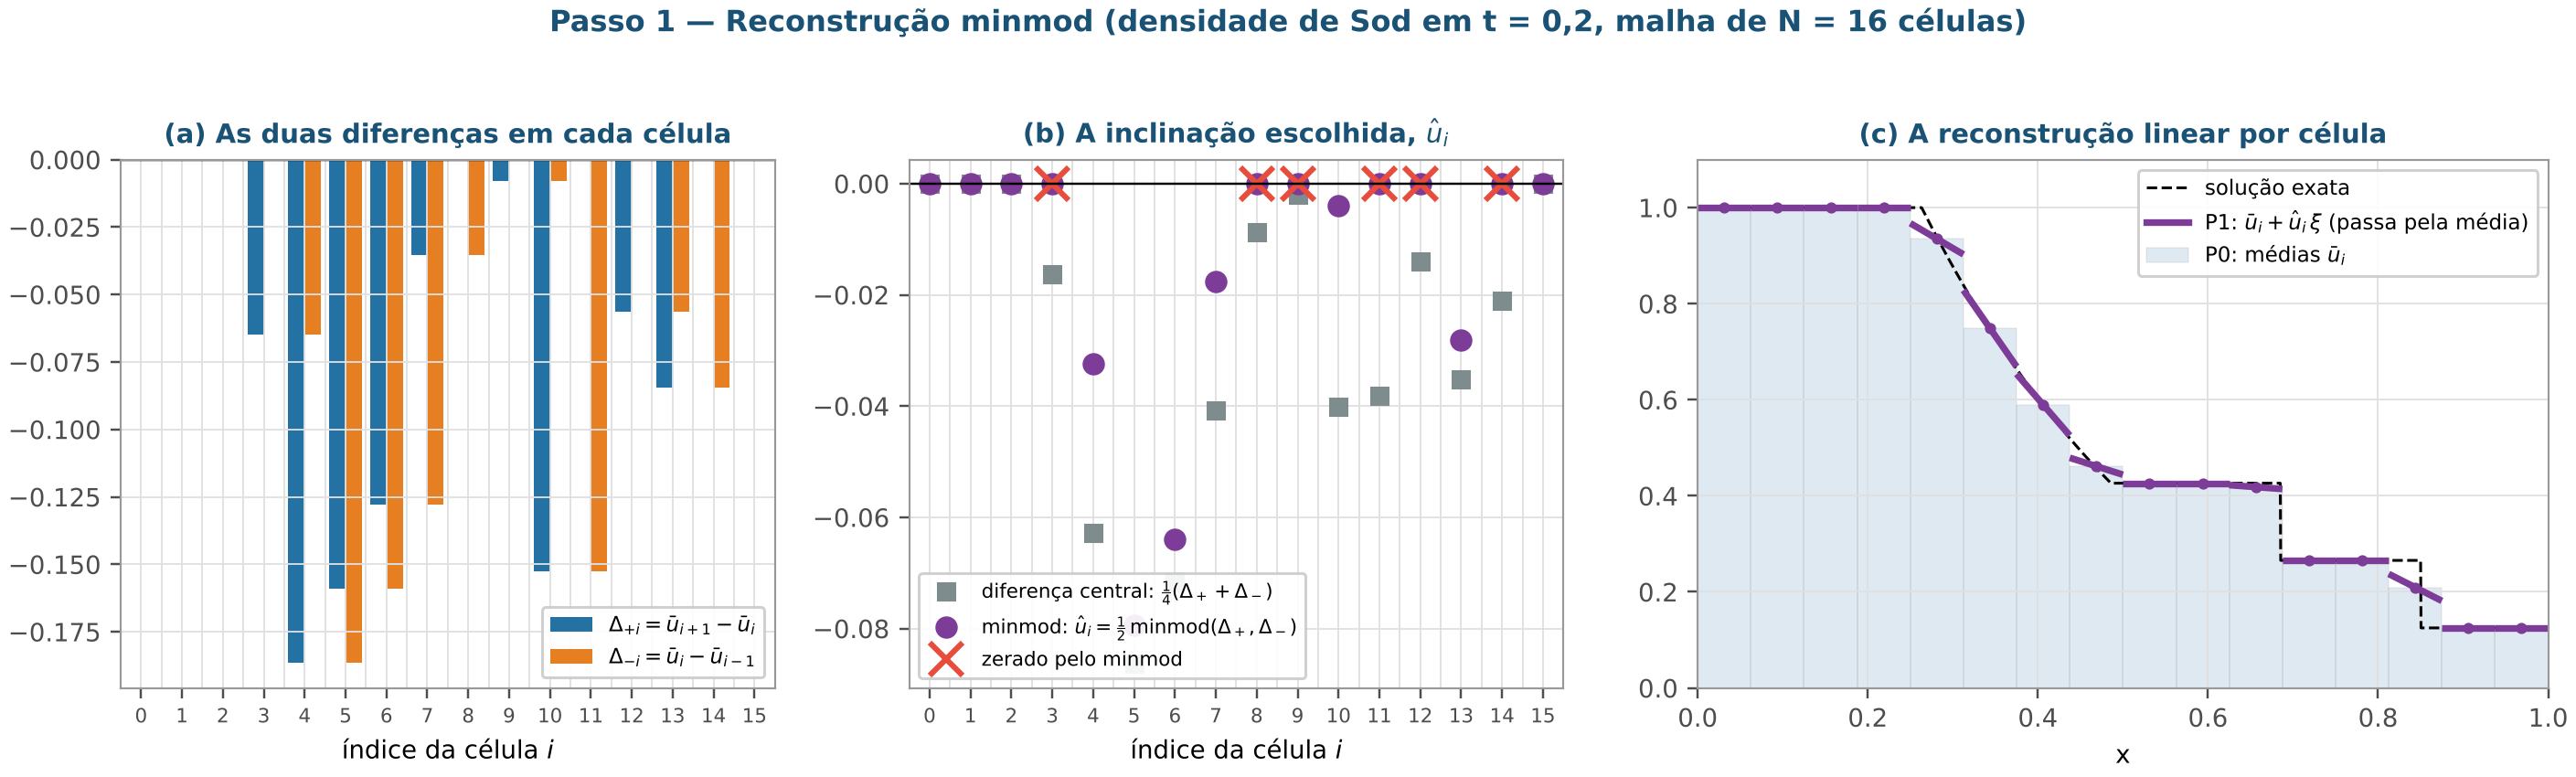
\includegraphics[width=\textwidth]{figs/fig2_minmod.png}
\caption{\textbf{Passo 1 em ação}, sobre as médias da densidade de Sod em $t=0{,}2$ (24 células). (a) As duas diferenças de cada célula, $\Delta_{+i}$ (azul) e $\Delta_{-i}$ (laranja); nos trechos constantes elas são nulas. (b) A inclinação escolhida: o minmod (círculos roxos) fica sempre com a menor das duas em módulo, enquanto a diferença central (quadrados cinza) fica com a média; as cruzes vermelhas marcam as células em que o minmod zerou a inclinação, porque um dos vizinhos é constante ou os sinais discordam, como nas duas células que contêm os saltos. (c) A reconstrução linear resultante (roxo) sobre as médias (azul-claro) e a solução exata (tracejada): nas regiões suaves a reta acompanha a curva; nas células dos saltos ela é horizontal.}
\label{fig:minmod}
\end{figure}

\subsection{Implementação}

\begin{lstlisting}[caption={Reconstrução minmod (Python). As células fantasma copiam o valor da vizinha (contorno transmissivo); U tem uma linha por variável conservada e uma coluna por célula.},label=lst:minmod]
def minmod(a, b):
    """Menor dos dois em modulo se os sinais coincidem; zero caso contrario."""
    same_sign = (a * b > 0)
    return np.where(same_sign, np.where(np.abs(a) < np.abs(b), a, b), 0.0)

def ghost(U):
    """Acrescenta uma celula fantasma de cada lado (copia da vizinha)."""
    return np.concatenate((U[:, :1], U, U[:, -1:]), axis=1)

def reconstruct(U):
    """Coeficiente u_hat_i de cada celula: valor de face = media +- u_hat."""
    Ug = ghost(U)
    delta_plus  = Ug[:, 2:]   - Ug[:, 1:-1]     # Delta_+ = u_{i+1} - u_i
    delta_minus = Ug[:, 1:-1] - Ug[:, :-2]      # Delta_- = u_i - u_{i-1}
    return 0.5 * minmod(delta_plus, delta_minus)
\end{lstlisting}

A reconstrução é feita \emph{componente a componente} nas variáveis conservadas ($\rho$, $\rho v$, $E$). É a escolha mais simples e a usada neste tutorial; variantes reconstroem nas variáveis primitivas ($\rho$, $v$, $p$) ou nas características, com resultados um pouco mais nítidos ao custo de mais álgebra.

% ================================================================ 5
\section{Passo 2: Estados nas interfaces}

Com a reconstrução feita, avaliamos $u_h$ nos dois lados de cada interface. Na interface $x_{i+1/2}$:
\begin{destaque}
\begin{align}
u^-_{i+1/2}&=\ub_i+\uh_i\qquad\ \ \text{(limite pela esquerda, }\xi=+1)\label{eq:um}\\
u^+_{i+1/2}&=\ub_{i+1}-\uh_{i+1}\quad\text{(limite pela direita, }\xi=-1)\label{eq:up}
\end{align}
\end{destaque}

Em geral, $u^-\neq u^+$ --- a solução é \textbf{descontínua} na interface. Isso é uma característica central do framework DG: cada célula ``não conversa'' com a vizinha diretamente. A comunicação acontece via o \textbf{fluxo numérico}, que resolve o ``conflito'' entre os dois valores.

Continuando o exemplo à mão da Seção~4.1: com $\ub_i=0{,}50$ e $\uh_i=0{,}05$, o lado esquerdo da face $x_{i+1/2}$ vale $u^-=0{,}55$. Se a célula seguinte tem $\ub_{i+1}=0{,}60$ e, digamos, $\uh_{i+1}=0{,}03$, o lado direito vale $u^+=0{,}57$. O salto na face é $0{,}02$, bem menor que o salto $0{,}10$ entre as médias. Essa é a diferença entre primeira e segunda ordem numa frase: \textbf{a reconstrução encolhe os saltos nas faces onde a solução é suave}; o fluxo numérico, que ``vê'' apenas o salto, passa a trabalhar quase como se a solução fosse contínua.

\begin{intuicao}
Os dois valores $u^-$ e $u^+$ definem um \textbf{problema de Riemann local} na interface --- exatamente o tipo de problema que Euler, Burgers e todas as leis de conservação hiperbólicas geram: dado um salto em $u$, o que acontece?

Na equação de Burgers, se $u^->u^+$, forma-se um choque; se $u^-<u^+$, uma rarefação. No sistema de Euler, a situação é mais rica: podem surgir até três ondas simultaneamente.
\end{intuicao}

\begin{figure}[htbp]
\centering
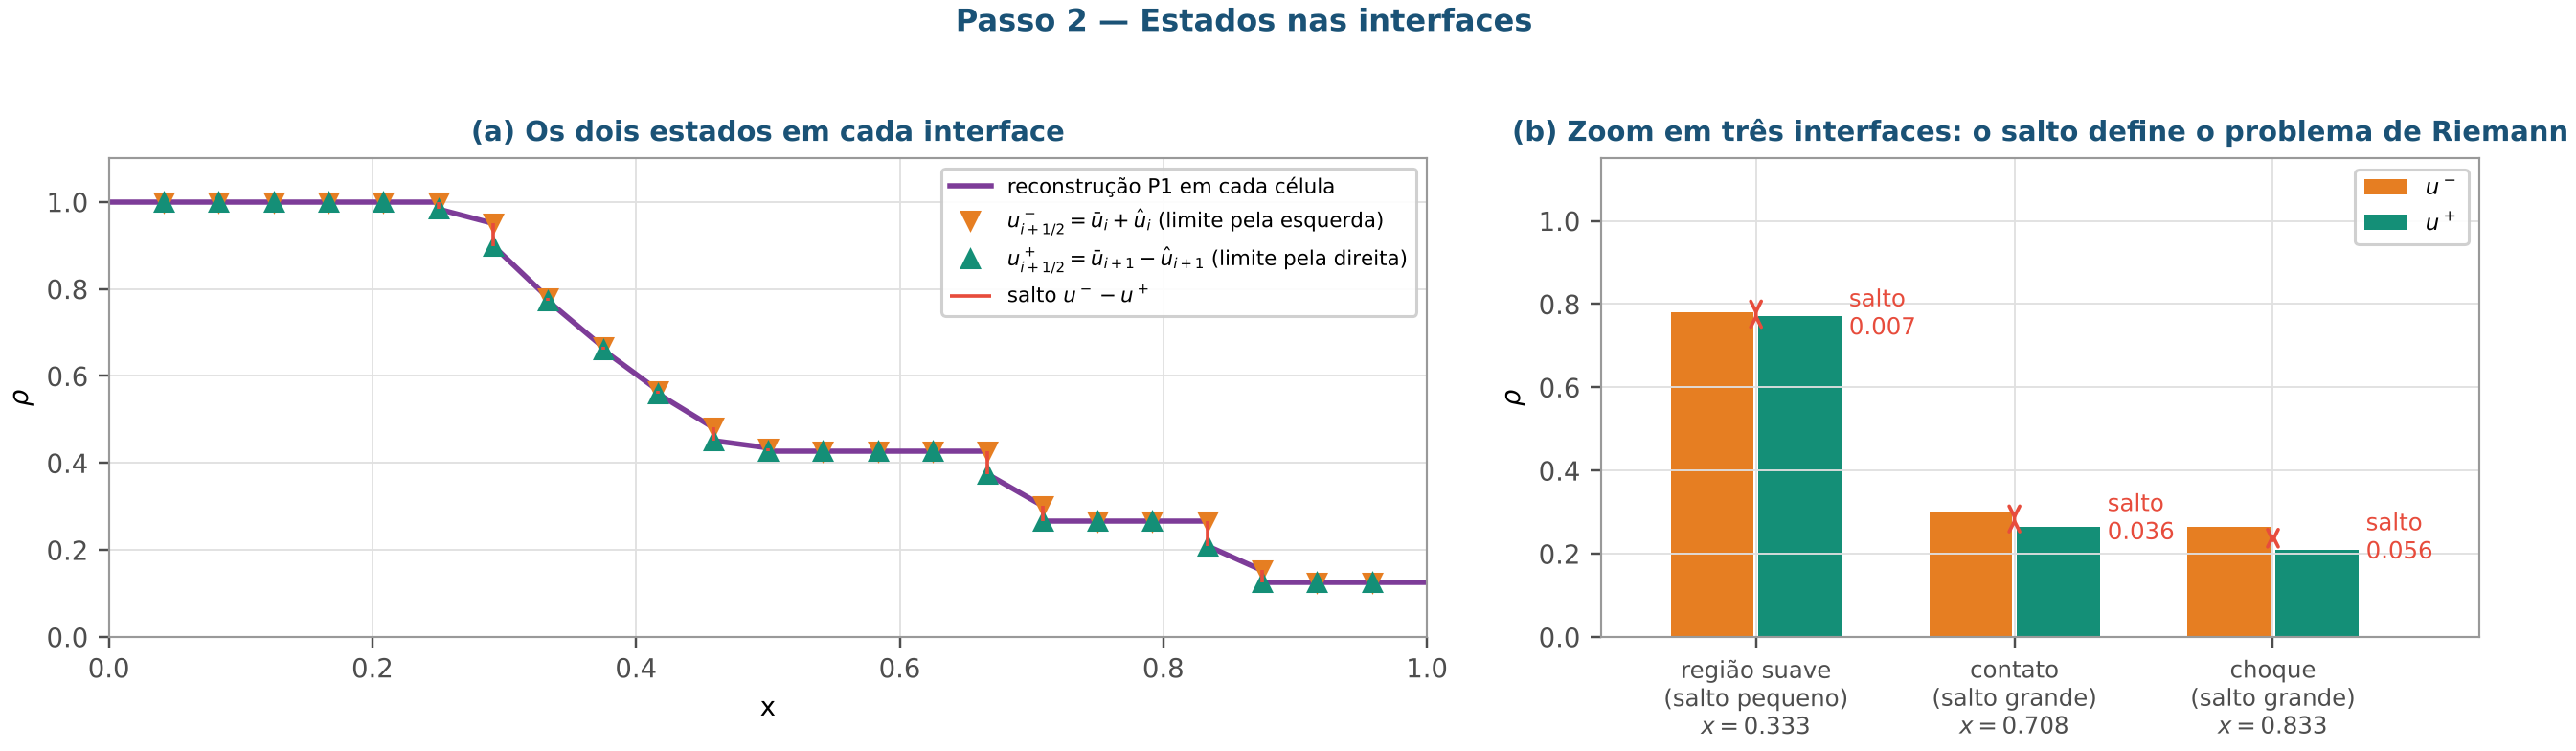
\includegraphics[width=\textwidth]{figs/fig3_interfaces.png}
\caption{\textbf{Passo 2.} Esquerda: a reconstrução P1 de cada célula (roxo) e os dois estados em cada interface, $u^-$ (triângulo laranja, vindo da célula da esquerda) e $u^+$ (triângulo verde, vindo da célula da direita); o segmento vermelho entre eles é o salto. Onde a solução é suave os dois triângulos quase coincidem; nas células do contato e do choque, em que o minmod zerou a inclinação, o salto é grande. Direita: zoom em três interfaces com os valores numéricos dos saltos; cada par $(u^-,u^+)$ é o dado de um problema de Riemann local.}
\label{fig:interfaces}
\end{figure}

% ================================================================ 6
\section{Passo 3: O fluxo numérico HLLC}

\subsection{O que é um fluxo numérico?}

O fluxo numérico $\fh_{i+1/2}=\fh(u^-_{i+1/2},u^+_{i+1/2})$ é uma função que, dados os dois estados na interface, retorna um \emph{único} valor de fluxo para usar em \eqref{eq:fv}. Ele é o coração do método: é ele que determina quanta ``coisa'' passa de uma célula para a outra.

Propriedades essenciais:
\begin{itemize}[leftmargin=2.5em,itemsep=3pt]
\item \textbf{Consistência}: $\fh(u,u)=f(u)$ (se não há salto, o fluxo numérico coincide com o físico);
\item \textbf{Upwinding}: a informação deve viajar na direção correta (respeitando as características).
\end{itemize}

A maneira mais fiel de obter esse valor é resolver exatamente o problema de Riemann da interface e ler a solução sobre a própria interface ($x/t=0$): é o \textbf{método de Godunov}. Para Euler isso custa uma iteração de Newton por interface e por passo. Os \emph{solvers aproximados}, como o HLLC, dão uma resposta quase tão boa com álgebra fechada. Todos eles podem ser escritos como ``média dos dois fluxos menos uma dissipação proporcional ao salto'': a arte está em dosar a dissipação de cada onda.

\subsection{A ideia do HLLC}

O HLLC (Harten--Lax--van Leer--Contact) é um \textbf{solver de Riemann aproximado} para sistemas. Ele assume que a solução do problema de Riemann local tem uma estrutura simplificada com \textbf{três ondas}:
\[
\begin{array}{c}
\toprule
\vu_L\ \xrightarrow{\ S_L\ }\ \vu_{*L}\ \xrightarrow{\ S_*\ }\ \vu_{*R}\ \xrightarrow{\ S_R\ }\ \vu_R\\
\bottomrule
\end{array}
\]
\begin{itemize}[leftmargin=2.5em,itemsep=3pt]
\item $S_L$, $S_R$: ondas externas (acústicas, no caso de Euler);
\item $S_*$: onda de contato (a ``Contact'' do HLLC) --- separa duas regiões que têm a mesma pressão e velocidade $S_*$, mas densidades diferentes.
\end{itemize}

Entre as ondas, a solução é suposta \emph{constante}: dois estados ``estrela'', $\vu_{*L}$ e $\vu_{*R}$. Eles não são chutados: saem das relações de salto (Rankine--Hugoniot) aplicadas através de $S_L$ e de $S_R$, com a exigência de que velocidade e pressão sejam as mesmas dos dois lados do contato. O resultado, para $K=L,R$, é
\begin{equation}\label{eq:estrela}
\vu_{*K}=\rho_K\,\frac{S_K-v_K}{S_K-S_*}
\begin{pmatrix}1\\[2pt] S_*\\[2pt] \dfrac{E_K}{\rho_K}+(S_*-v_K)\Big(S_*+\dfrac{p_K}{\rho_K\,(S_K-v_K)}\Big)\end{pmatrix}.
\end{equation}
O fator $\rho_K(S_K-v_K)/(S_K-S_*)$ é a conservação de massa através da onda $S_K$ escrita no referencial da onda: o que entra por um lado com velocidade relativa $S_K-v_K$ sai pelo outro com velocidade relativa $S_K-S_*$.

\begin{intuicao}
O HLL original (sem o ``C'') assume apenas duas ondas e um único estado intermediário. Isso é suficiente para capturar choques e rarefações, mas \emph{borra completamente} as descontinuidades de contato (interfaces entre materiais, por exemplo). O HLLC adiciona a onda de contato, resolvendo esse problema.

O motivo é simples: num contato só a densidade salta, com $p$ e $v$ contínuos. O HLL mistura os dois lados num estado médio único e trata esse salto como se fosse uma onda acústica, dissipando-o com a velocidade do som. O HLLC coloca o salto de densidade na onda $S_*$, que viaja com o fluido, dissipando-o só com $|S_*|$: numa frente de contato lenta, a diferença entre borrar e não borrar.
\end{intuicao}

\subsection{A fórmula}

O fluxo HLLC depende da posição relativa da interface em relação às três ondas:
\begin{destaque}
\begin{equation}\label{eq:hllc}
\fh_{i+1/2}=
\begin{cases}
\vf_L & \text{se } S_L>0\\
\vf_{*L}=\vf_L+S_L(\vu_{*L}-\vu_L) & \text{se } S_L\le0<S_*\\
\vf_{*R}=\vf_R+S_R(\vu_{*R}-\vu_R) & \text{se } S_*\le0\le S_R\\
\vf_R & \text{se } S_R<0
\end{cases}
\end{equation}
\end{destaque}
As velocidades de onda são estimadas via Davis:
\begin{equation}\label{eq:davis}
S_L=\min(v_L-a_L,\ v_R-a_R),\qquad S_R=\max(v_L+a_L,\ v_R+a_R)
\end{equation}
e a velocidade de contato:
\begin{equation}\label{eq:sstar}
S_*=\frac{p_R-p_L+\rho_Lv_L(S_L-v_L)-\rho_Rv_R(S_R-v_R)}{\rho_L(S_L-v_L)-\rho_R(S_R-v_R)}
\end{equation}

Por que as fórmulas dos ramos intermediários têm a forma $\vf_K+S_K(\vu_{*K}-\vu_K)$? É de novo Rankine--Hugoniot: através de uma onda de velocidade $S$, o salto de fluxo é $S$ vezes o salto de estado. Partindo de $\vf_L$ e atravessando a onda $S_L$ chega-se ao fluxo da região estrela esquerda. A estimativa de Davis \eqref{eq:davis} escolhe para $S_L$ e $S_R$ a menor e a maior velocidade acústica dos dois estados: com isso as ondas externas do modelo são pelo menos tão rápidas quanto as verdadeiras, o que garante a dissipação necessária para que nenhum estado não físico apareça. A fórmula \eqref{eq:sstar} é o que resulta de impor que o momento se conserve entre $S_L$ e $S_R$ com $v=S_*$ e $p$ iguais nas duas regiões estrela.

\begin{intuicao}
Os quatro ramos de \eqref{eq:hllc} correspondem a quatro situações físicas: (i) todas as ondas vão para a direita (escoamento supersônico para a direita); (ii) a interface está entre $S_L$ e $S_*$ (região estrela esquerda); (iii) a interface está entre $S_*$ e $S_R$ (região estrela direita); (iv) todas as ondas vão para a esquerda.

A pergunta que a fórmula responde é sempre a mesma: ``olhando a interface, $x/t=0$, no diagrama de ondas, em qual das quatro regiões ela está?'' O fluxo numérico é o fluxo da região em que a interface cai. Na interface central do tubo de Sod no instante inicial, $S_L=-1{,}18$, $S_*=0{,}68$ e $S_R=1{,}18$: a interface está na região estrela esquerda e vale o ramo (ii).
\end{intuicao}

\begin{figure}[htbp]
\centering
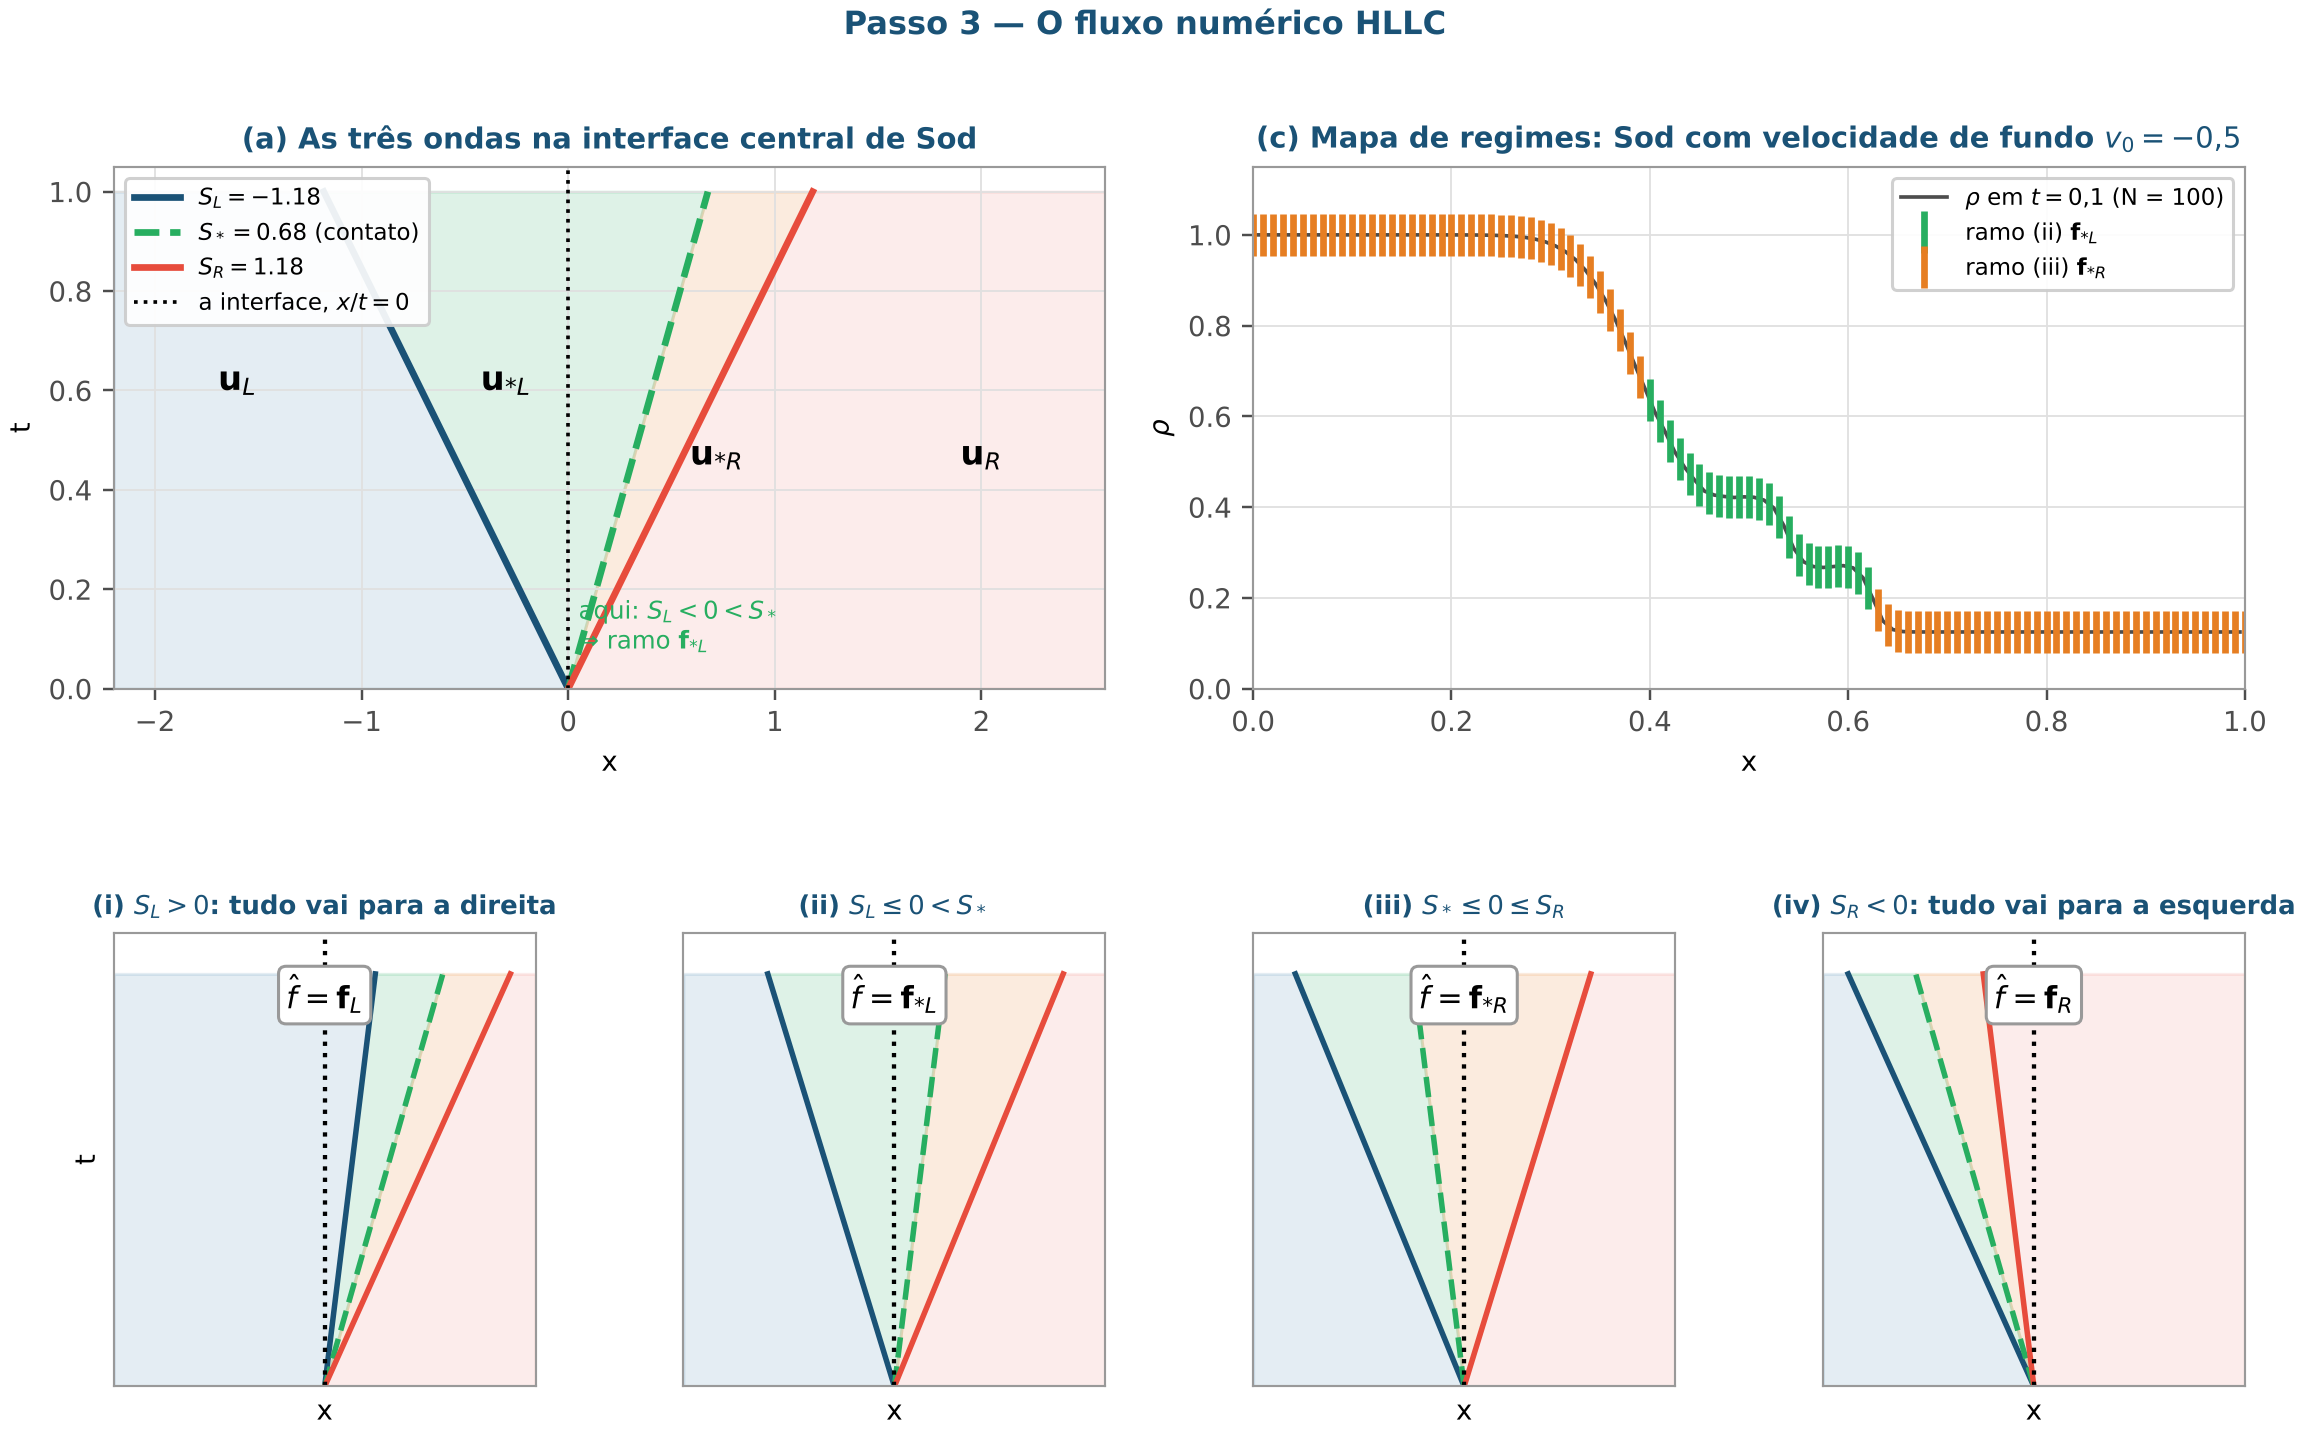
\includegraphics[width=\textwidth]{figs/fig4_hllc.png}
\caption{\textbf{Passo 3.} (a) Diagrama espaço-tempo das três ondas do HLLC para a interface central do tubo de Sod no instante inicial; as quatro regiões coloridas são os quatro estados; a linha pontilhada é a interface. (b) Os quatro ramos de \eqref{eq:hllc}: o que muda de um para outro é a região em que a interface cai. (c) Mapa de regimes numa simulação real: o tubo de Sod com uma velocidade de fundo $v_0=-0{,}5$ em $t=0{,}1$; cada traço vertical marca uma interface, colorida pelo ramo usado. Onde o gás anda para a esquerda a interface cai na região estrela direita (laranja, ramo iii); onde a rarefação o acelera para a direita, na região estrela esquerda (verde, ramo ii). Sem velocidade de fundo todas as interfaces usariam o ramo (ii), por isso o mapa do problema de Sod puro é pouco instrutivo.}
\label{fig:hllc}
\end{figure}

\subsection{Implementação}

\begin{lstlisting}[caption={Fluxo HLLC vetorizado (trechos-chave). As funções conserved\_to\_primitive, sound\_speed e euler\_flux implementam \eqref{eq:eos} e \eqref{eq:euler}.},label=lst:hllc]
def hllc_flux(uL, uR):
    rhoL, vL, pL = conserved_to_primitive(uL)
    rhoR, vR, pR = conserved_to_primitive(uR)
    aL, aR = sound_speed(rhoL, pL), sound_speed(rhoR, pR)
    fL, fR = euler_flux(uL), euler_flux(uR)

    # Velocidades de onda (Davis)
    SL = np.minimum(vL - aL, vR - aR)
    SR = np.maximum(vL + aL, vR + aR)

    # Onda de contato
    num = pR - pL + rhoL*vL*(SL-vL) - rhoR*vR*(SR-vR)
    den = rhoL*(SL - vL) - rhoR*(SR - vR)
    S_star = num / den

    # Estados estrela, eq. (14)
    def star(u, rho, v, p, S):
        fac = rho * (S - v) / (S - S_star)
        return np.array([fac, fac*S_star,
                         fac*(u[2]/rho + (S_star - v)*(S_star + p/(rho*(S - v))))])
    u_starL = star(uL, rhoL, vL, pL, SL)
    u_starR = star(uR, rhoR, vR, pR, SR)

    # Montar fluxo por regiao
    F = np.where(SL >= 0, fL,
        np.where(S_star >= 0,
                 fL + SL*(u_starL - uL),      # regiao *L
        np.where(SR >= 0,
                 fR + SR*(u_starR - uR),      # regiao *R
                 fR)))                        # regiao R
    return F
\end{lstlisting}

% ================================================================ 7
\section{Passo 4: Atualização temporal}

\subsection{O operador espacial}

Juntando os passos anteriores, definimos o operador espacial:
\begin{equation}\label{eq:L}
L(\ub)_i=-\frac{1}{\Delta x}\Big[\fh_{i+1/2}-\fh_{i-1/2}\Big]
\end{equation}
de modo que $\frac{d\ub_i}{dt}=L(\ub)_i$. Cada avaliação de $L$ envolve o pipeline completo: reconstrução $\to$ interfaces $\to$ HLLC.

O que sobrou é um sistema de $3N$ equações diferenciais ordinárias no tempo, uma por variável conservada e por célula: é a abordagem conhecida como \emph{método das linhas}. Qualquer integrador de EDOs serve em princípio; a escolha entre explícito e implícito é a decisão que resta.

\subsection{BDF2 (\emph{Backward Differentiation Formula} de 2ª ordem)}

Para integrar no tempo, utilizamos o método BDF2 (totalmente implícito), que aproxima a derivada temporal em $t^{n+1}$ usando os dois instantes anteriores:
\begin{destaque}
\begin{equation}\label{eq:bdf2}
\frac{3\,\ub^{n+1}-4\,\ub^n+\ub^{n-1}}{2\,\Delta t}=L(\ub^{n+1})
\end{equation}
\end{destaque}

A fórmula vem de um argumento de interpolação: faça passar uma parábola pelos três valores $\ub^{n-1}$, $\ub^n$ e $\ub^{n+1}$ (igualmente espaçados em $\Delta t$) e derive-a no último ponto. O resultado é o lado esquerdo de \eqref{eq:bdf2}; os pesos $3$, $-4$ e $1$ são os da derivada dessa parábola. Como a parábola reproduz exatamente qualquer polinômio de grau $2$, o erro é $O(\Delta t^2)$: segunda ordem no tempo, compatível com a segunda ordem no espaço.

Rearranjando, o problema a cada passo de tempo é encontrar $\ub^{n+1}$ tal que o \textbf{resíduo} se anule:
\begin{equation}\label{eq:residuo}
\mathbf{F}(\ub^{n+1})\equiv3\,\ub^{n+1}-4\,\ub^n+\ub^{n-1}-2\,\Delta t\,L(\ub^{n+1})=\mathbf{0}
\end{equation}
Este é um sistema \textbf{não-linear} (pois $L$ depende de $\ub^{n+1}$ via reconstrução + HLLC) e é resolvido iterativamente pelo método de Newton:
\begin{equation}\label{eq:newton}
\mathbb{J}^{(k)}\,\delta\ub=-\mathbf{F}(\ub^{(k)}),\qquad \ub^{(k+1)}=\ub^{(k)}+\delta\ub
\end{equation}
onde $\mathbb{J}^{(k)}=\partial\mathbf{F}/\partial\ub\,\big|^{(k)}$ é a matriz Jacobiana. Na prática, pode-se utilizar o método \emph{Jacobian-Free Newton--Krylov} (JFNK) para evitar a montagem explícita de $\mathbb{J}$.

A ideia do JFNK cabe em uma linha. O método de Krylov (GMRES) que resolve o sistema linear \eqref{eq:newton} nunca pede a matriz $\mathbb{J}$ inteira: pede apenas produtos $\mathbb{J}\mathbf{w}$ para vetores $\mathbf{w}$ que ele próprio escolhe. E um produto Jacobiana-vetor é uma derivada direcional, que se aproxima por diferença finita com \emph{uma} avaliação extra do resíduo:
\begin{equation}\label{eq:jfnk}
\mathbb{J}\,\mathbf{w}\approx\frac{\mathbf{F}(\ub+\epsilon\,\mathbf{w})-\mathbf{F}(\ub)}{\epsilon},\qquad \epsilon\sim10^{-7}.
\end{equation}
Assim a única coisa que o programador escreve é a função resíduo; a Jacobiana, com os seus $(3N)^2$ coeficientes e as suas derivadas do minmod e do HLLC, nunca é montada.

\begin{atencao}
\textbf{Inicialização:} No primeiro passo de tempo ($n=0\to1$), a solução $\ub^{-1}$ não existe. Usa-se então o \emph{Backward Euler} (BDF1, primeira ordem):
\[
\frac{\ub^1-\ub^0}{\Delta t}=L(\ub^1)
\]
A partir de $n\ge1$, o BDF2 é utilizado normalmente.

\textbf{Passo constante:} os pesos $3$, $-4$ e $1$ valem para $\Delta t$ constante. Se o passo mudar de um nível para outro, os coeficientes mudam (BDF2 de passo variável). Neste tutorial fixamos $\Delta t$ a partir do estado inicial e ajustamos o último passo para terminar exatamente em $t_{\text{final}}$.
\end{atencao}

\begin{intuicao}
O BDF2 é um método \textbf{implícito} e \textbf{A-estável}, o que significa que não há restrição de CFL para estabilidade --- o passo de tempo pode ser escolhido com base na \emph{precisão} desejada, não na estabilidade. Isso é essencial em problemas com escalas de tempo díspares (por exemplo, ondas acústicas rápidas e transporte lento), onde métodos explícitos exigiriam passos de tempo proibitivamente pequenos.

O preço a pagar é a necessidade de resolver um sistema não-linear a cada passo de tempo, o que torna cada passo mais caro do que num método explícito. Porém, a possibilidade de usar $\Delta t$ muito maiores frequentemente compensa esse custo.
\end{intuicao}

A escolha do passo de tempo é guiada pela precisão temporal desejada. Uma regra prática é:
\begin{equation}\label{eq:cfl}
\Delta t=\mathrm{CFL}\cdot\frac{\Delta x}{\max_i(|v_i|+a_i)}
\end{equation}
com CFL tipicamente entre 1 e 100 (dependendo da rigidez do problema), em contraste com o CFL $\le1$ dos métodos explícitos.

\begin{atencao}
\textbf{Estável não quer dizer preciso.} Com $\mathrm{CFL}=5$ o método não explode, mas a informação atravessa cinco células por passo e o BDF2 espalha choques e contatos por várias células, como a Figura~\ref{fig:convergencia}(c) mostra. Para um problema dominado por ondas rápidas, como o tubo de Sod, o passo grande desperdiça a resolução espacial; é nos transientes lentos, em que as ondas acústicas não interessam, que o CFL alto compensa. Nos resultados deste tutorial usamos $\mathrm{CFL}=1$.

\textbf{O ``Newton simplificado'' do Listing~\ref{lst:bdf2} só converge com passos pequenos.} Trocar a Jacobiana por $3\,\mathbb{I}$ transforma \eqref{eq:newton} numa iteração de ponto fixo, $\ub\leftarrow\ub-\mathbf{F}/3$, que contrai apenas se $\tfrac23\Delta t\,\|\partial L/\partial\ub\|<1$. Como $\|\partial L/\partial\ub\|\approx2\max(|v|+a)/\Delta x$, a condição é $\mathrm{CFL}<3/4$. Com $\mathrm{CFL}=5$ a iteração diverge em poucos passos (Figura~\ref{fig:tempo}c); com $\mathrm{CFL}=0{,}5$ ela converge devagar. O JFNK converge em meia dúzia de iterações nos dois casos. Em resumo: o ponto fixo serve para entender a estrutura do código, o JFNK é o que se usa.
\end{atencao}

\begin{figure}[htbp]
\centering
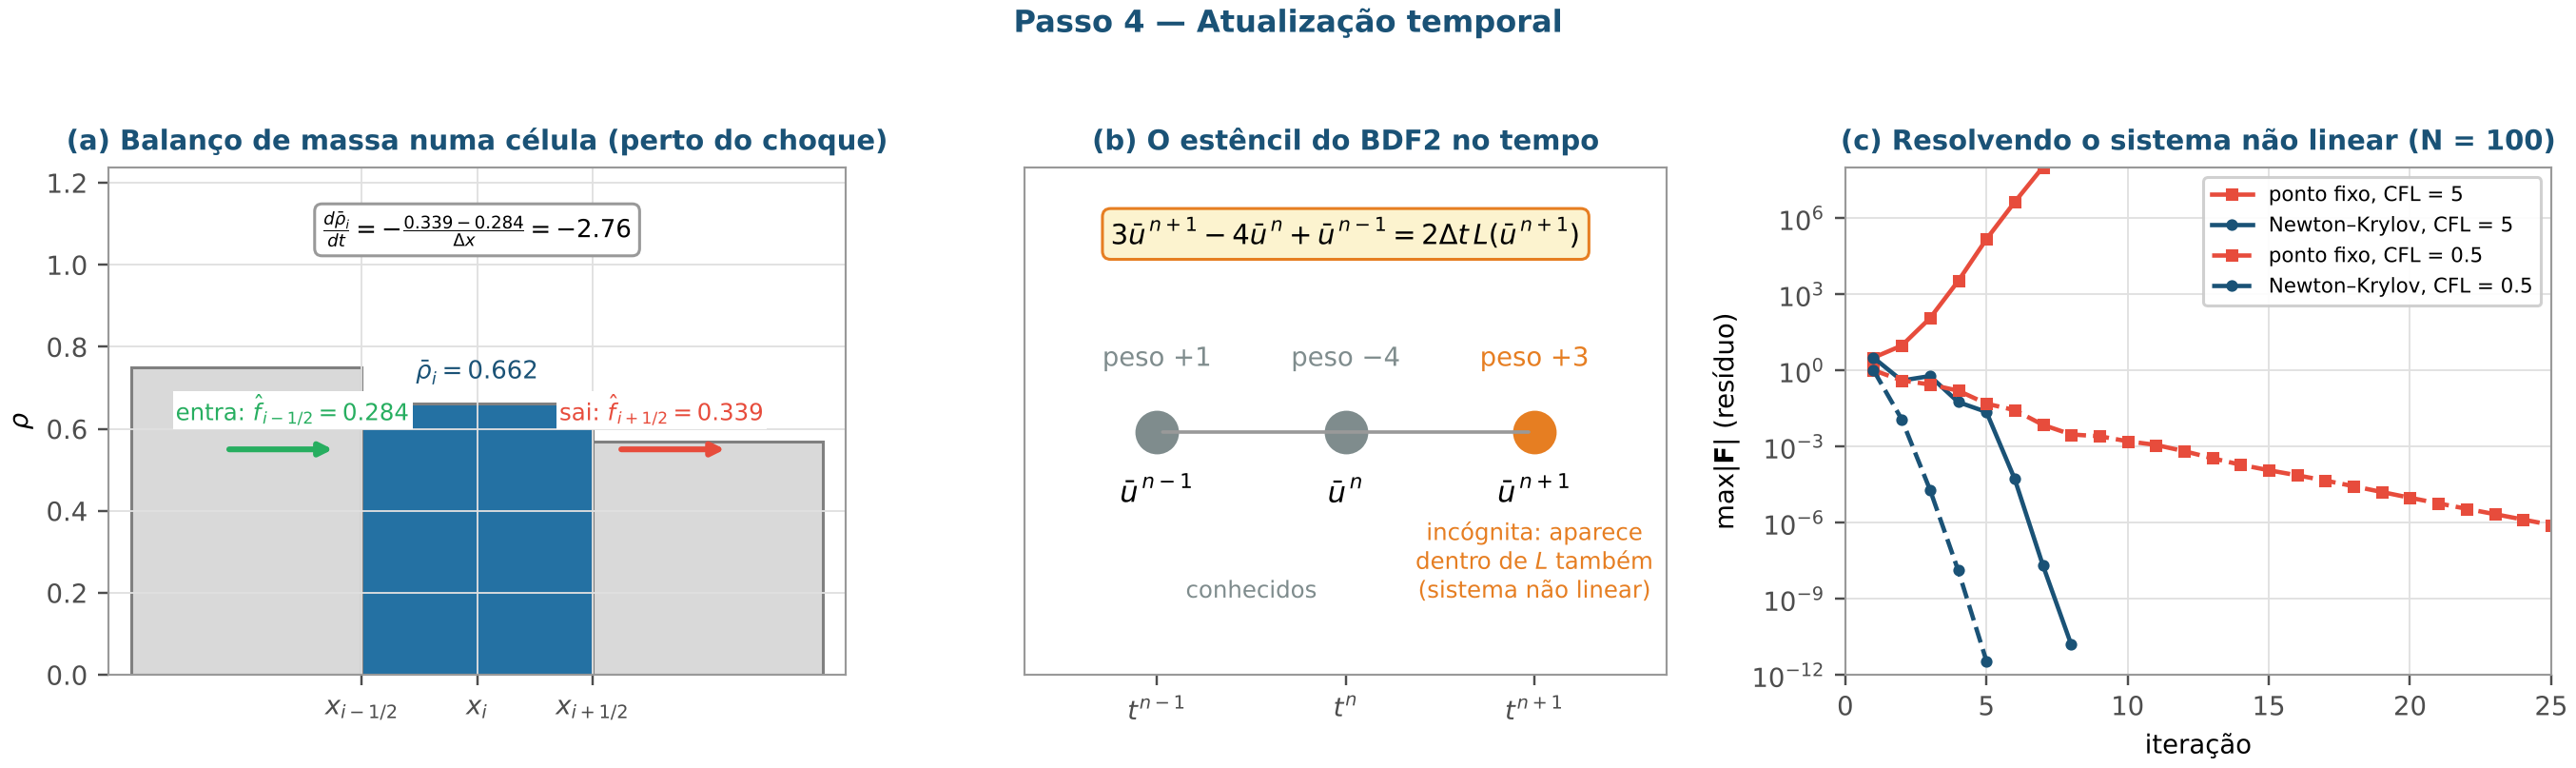
\includegraphics[width=\textwidth]{figs/fig5_tempo.png}
\caption{\textbf{Passo 4.} (a) Balanço de massa numa célula logo à esquerda do choque de Sod ($t=0{,}1$, $N=50$): entra $\fh_{i-1/2}$ pela esquerda, sai $\fh_{i+1/2}$ pela direita e a diferença, dividida por $\Delta x$, é a taxa de variação da média --- aqui negativa, porque o choque está deixando a célula para trás. (b) O estêncil do BDF2: dois níveis conhecidos, com pesos $-4$ e $+1$, mais a incógnita $\ub^{n+1}$ com peso $3$, que aparece também dentro de $L$: daí o sistema não linear. (c) Resíduo por iteração no primeiro passo BDF2 ($N=100$): o Newton--Krylov converge até $10^{-10}$ em menos de dez iterações para $\mathrm{CFL}=0{,}5$ e $\mathrm{CFL}=5$; a iteração de ponto fixo converge devagar com $\mathrm{CFL}=0{,}5$ e diverge com $\mathrm{CFL}=5$.}
\label{fig:tempo}
\end{figure}

\subsection{Implementação}

\begin{lstlisting}[caption={Avanço temporal BDF2 com iterações de Newton (Python), versão mínima. Lê-se bem, mas a aproximação $\mathbb{J}\approx3\,\mathbb{I}$ só converge para $\mathrm{CFL}<3/4$ (veja a caixa de atenção acima).},label=lst:bdf2]
def bdf2_step(U_n, U_nm1, dx, dt, tol=1e-10, max_iter=50):
    """Um passo BDF2: resolve 3*U - 4*U_n + U_nm1 - 2*dt*L(U) = 0."""
    U = U_n.copy()          # chute inicial
    for k in range(max_iter):
        L = compute_rhs(U, dx)
        F = 3*U - 4*U_n + U_nm1 - 2*dt*L      # residuo
        if np.max(np.abs(F)) < tol:
            break
        # Jacobiana aproximada (diagonal): dF/dU ~ 3*I  -> ponto fixo
        dU = -F / 3.0
        U = U + dU
    return U

def backward_euler_step(U_n, dx, dt, tol=1e-10, max_iter=50):
    """Primeiro passo (BDF1): resolve U - U_n - dt*L(U) = 0."""
    U = U_n.copy()
    for k in range(max_iter):
        L = compute_rhs(U, dx)
        F = U - U_n - dt*L
        if np.max(np.abs(F)) < tol:
            break
        dU = -F / 1.0
        U = U + dU
    return U
\end{lstlisting}

\begin{lstlisting}[caption={A mesma etapa com Newton--Krylov sem Jacobiana (JFNK). O produto Jacobiana-vetor é a diferença finita \eqref{eq:jfnk}; o GMRES resolve o sistema linear de cada iteração de Newton de forma aproximada (resíduo linear relativo $10^{-3}$ basta).},label=lst:jfnk]
from scipy.sparse.linalg import LinearOperator, gmres

def newton_krylov_step(U_n, U_nm1, dx, dt, tol=1e-10, max_iter=50):
    """Resolve F(U) = 0 (BDF2, ou BDF1 se U_nm1 is None) por JFNK."""
    shape = U_n.shape
    def residual(x):
        U = x.reshape(shape)
        L = compute_rhs(U, dx)
        if U_nm1 is None:
            return (U - U_n - dt*L).ravel()
        return (3*U - 4*U_n + U_nm1 - 2*dt*L).ravel()
    x = U_n.ravel().copy()
    for k in range(max_iter):
        F = residual(x)
        if np.max(np.abs(F)) < tol:
            break
        eps = 1e-7 * max(1.0, np.linalg.norm(x))
        def Jv(w):                       # produto Jacobiana-vetor por diferenca finita
            nw = np.linalg.norm(w)
            if nw == 0.0:
                return np.zeros_like(w)
            return (residual(x + (eps/nw)*w) - F) / (eps/nw)
        J = LinearOperator((x.size, x.size), matvec=Jv, dtype=float)
        dx_newton, info = gmres(J, -F, rtol=1e-3, restart=60, maxiter=200)
        x = x + dx_newton
    return x.reshape(shape)
\end{lstlisting}

% ================================================================ 8
\section{O pipeline completo}

Resumindo, para \textbf{cada iteração de Newton} dentro de um passo BDF2:

\begin{center}
\renewcommand{\arraystretch}{1.4}
\begin{tabular}{@{}c l l@{}}
\toprule
\textbf{Passo} & \textbf{O que faz} & \textbf{Onde está ilustrado}\\
\midrule
\textcircled{1} Reconstrução & $\uh_i=\tfrac12\,\mathrm{minmod}(\Delta_+,\Delta_-)$ & Figura~\ref{fig:minmod}: retas roxas (P1)\\
\textcircled{2} Interfaces & $u^-=\ub_i+\uh_i$,\ \ $u^+=\ub_{i+1}-\uh_{i+1}$ & Figura~\ref{fig:interfaces}: triângulos $u^-$, $u^+$\\
\textcircled{3} Fluxo HLLC & $\fh=\mathrm{HLLC}(u^-,u^+)$ & Figura~\ref{fig:hllc}: ramos e regimes\\
\textcircled{4} Atualização BDF2 & $3\ub^{n+1}-4\ub^n+\ub^{n-1}=2\Delta t\,L(\ub^{n+1})$ & Figura~\ref{fig:tempo}: balanço e estêncil\\
\bottomrule
\end{tabular}
\end{center}

Os passos \textcircled{1}--\textcircled{3} são executados a cada avaliação do operador $L(\ub)$, ou seja, em cada iteração de Newton do passo \textcircled{4}. A reconstrução minmod é refeita com os dados mais recentes da iteração corrente. Num passo com oito iterações de Newton e, digamos, vinte produtos Jacobiana-vetor por iteração, o operador $L$ é avaliado perto de duzentas vezes: é o custo do implícito, pago em troca da liberdade no passo de tempo.

\begin{lstlisting}[caption={O pipeline completo em Python. O passo de tempo é fixado uma vez, a partir do estado inicial; é ajustado para terminar exatamente em t\_final.},label=lst:pipeline]
def compute_rhs(U, dx):
    """Operador espacial L(u): reconstrucao -> interfaces -> HLLC."""
    S = reconstruct(U)                       # Passo 1
    uL, uR = interface_states(U, S)          # Passo 2 (inclui as faces de contorno)
    F = hllc_flux(uL, uR)                    # Passo 3
    return -(F[:, 1:] - F[:, :-1]) / dx      # uma face a mais que celulas

def time_advance(U, dx, t_final, CFL=1.0):
    """Avanco temporal: BDF1 no primeiro passo, BDF2 nos demais, passo constante."""
    rho, v, p = conserved_to_primitive(U)
    dt = CFL * dx / np.max(np.abs(v) + sound_speed(rho, p))
    n_steps = int(np.ceil(t_final / dt))
    dt = t_final / n_steps                   # termina exatamente em t_final
    U_nm1 = None                             # nao existe no primeiro passo
    for n in range(n_steps):
        U_new = newton_krylov_step(U, U_nm1, dx, dt)   # BDF1 se U_nm1 is None
        U_nm1, U = U, U_new
    return U
\end{lstlisting}

% ================================================================ 9
\section{Resultados: tubo de choque de Sod}

O teste canônico para métodos de captura de choque é o \textbf{tubo de choque de Sod}: um tubo com gás em alta pressão à esquerda e baixa pressão à direita, separados por um diafragma em $x=0{,}5$:
\[
(\rho,v,p)=
\begin{cases}
(1{,}0,\ 0,\ 1{,}0) & x<0{,}5\\
(0{,}125,\ 0,\ 0{,}1) & x\ge0{,}5
\end{cases}
\]
A solução exata em $t=0{,}2$ contém três estruturas distintas:
\begin{enumerate}[leftmargin=2.5em,itemsep=3pt]
\item Uma \textbf{onda de rarefação} (suave) propagando-se para a esquerda --- aqui o método opera em segunda ordem;
\item Uma \textbf{descontinuidade de contato} (salto em $\rho$ mas não em $p$) --- é onde o ``C'' do HLLC faz diferença;
\item Um \textbf{choque} propagando-se para a direita --- aqui o minmod degenera para P0 e o método captura o choque sem oscilações.
\end{enumerate}

A solução exata é conhecida: a pressão e a velocidade entre as ondas valem $p^*=0{,}303$ e $v^*=0{,}927$, a cabeça da rarefação viaja a $-1{,}18$, o contato a $0{,}93$ e o choque a $1{,}75$. Como o choque é a onda mais rápida, em $t=0{,}2$ ele está em $x=0{,}85$, o contato em $x=0{,}69$ e a rarefação ocupa $0{,}26<x<0{,}49$. É com essa solução que comparamos os resultados numéricos.

\begin{figure}[htbp]
\centering
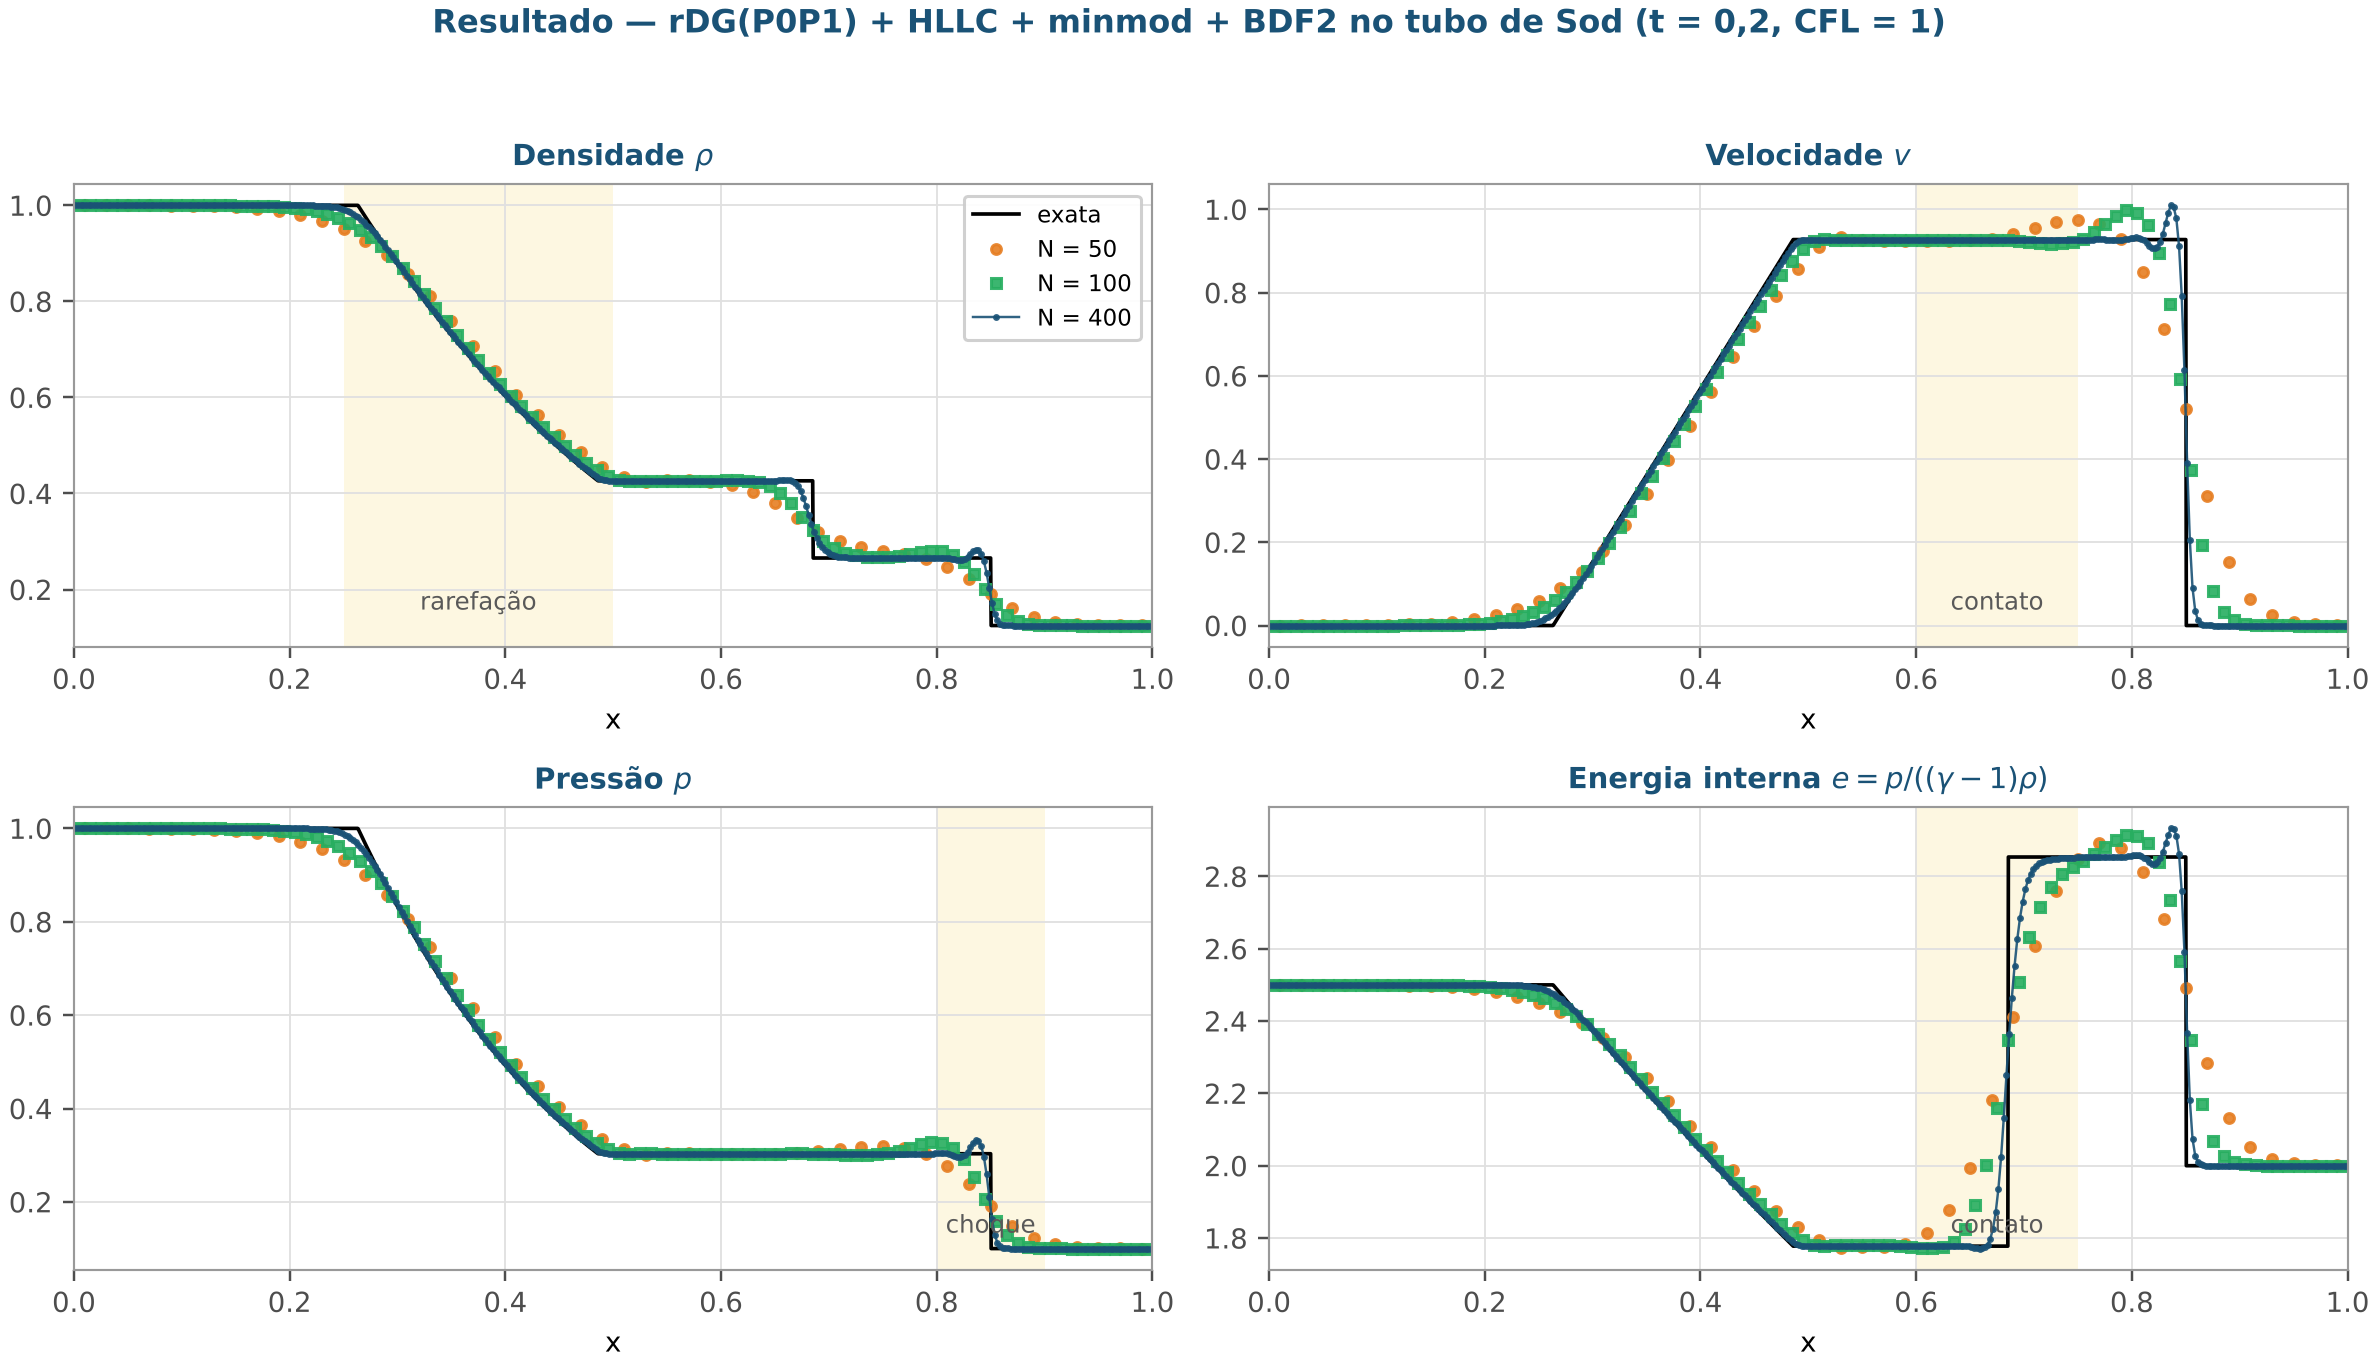
\includegraphics[width=\textwidth]{figs/fig6_sod.png}
\caption{Resultado do rDG(P0P1) + HLLC + minmod + BDF2 para o problema de Sod ($t=0{,}2$, $\mathrm{CFL}=1$) com três resoluções, nas quatro variáveis de interesse. A convergência com o refino da malha é visível em todas as estruturas: rarefação (esquerda), contato (centro) e choque (direita). O choque ocupa duas ou três células em qualquer malha; o contato é a estrutura mais borrada, como esperado; a energia interna, que o salta com amplitude grande, é a variável em que isso mais aparece. O pequeno sobressalto de velocidade e pressão logo atrás do choque é o erro de partida do BDF2 no instante inicial, quando o salto ainda ocupa uma célula.}
\label{fig:sod}
\end{figure}

\subsection{Convergência com a malha}

Olhar os perfis convence; medir o erro convence mais. A Tabela~\ref{tab:conv} e a Figura~\ref{fig:convergencia} mostram o erro $L^1$ da densidade, $E_N=\Delta x\sum_i|\bar\rho_i-\bar\rho_i^{\text{exata}}|$, para o método sem reconstrução (P0, primeira ordem) e com reconstrução minmod (rDG(P0P1)), em dois problemas: uma onda de densidade suave e periódica, $\rho_0(x)=1+0{,}2\,\sin(2\pi x)$ com $v=1$ e $p=1$, transportada por uma volta inteira, e o tubo de Sod.

\begin{table}[htbp]
\centering\small
\caption{Erro $L^1$ da densidade e razão entre erros ao dobrar $N$ (ordem $=\log_2$ da razão). Onda de densidade em $t=1$ e Sod em $t=0{,}2$, ambos com $\mathrm{CFL}=1$.}
\label{tab:conv}
\begin{tabular}{@{}r cc cc@{}}
\toprule
& \multicolumn{2}{c}{onda de densidade (suave)} & \multicolumn{2}{c}{Sod (com saltos)}\\
\cmidrule(lr){2-3}\cmidrule(lr){4-5}
$N$ & P0 & rDG(P0P1) & P0 & rDG(P0P1)\\
\midrule
20  & $7{,}97\times10^{-2}$ & $1{,}98\times10^{-2}$ & -- & --\\
40  & $4{,}96\times10^{-2}$ (1,6) & $8{,}60\times10^{-3}$ (2,3) & -- & --\\
50  & -- & -- & $3{,}05\times10^{-2}$ & $1{,}71\times10^{-2}$\\
80  & $2{,}79\times10^{-2}$ (1,8) & $2{,}55\times10^{-3}$ (3,4) & -- & --\\
100 & -- & -- & $2{,}10\times10^{-2}$ (1,5) & $9{,}94\times10^{-3}$ (1,7)\\
160 & $1{,}48\times10^{-2}$ (1,9) & $7{,}29\times10^{-4}$ (3,5) & -- & --\\
200 & -- & -- & $1{,}35\times10^{-2}$ (1,6) & $5{,}68\times10^{-3}$ (1,8)\\
320 & $7{,}62\times10^{-3}$ (1,9) & $1{,}98\times10^{-4}$ (3,7) & -- & --\\
400 & -- & -- & $8{,}45\times10^{-3}$ (1,6) & $3{,}06\times10^{-3}$ (1,9)\\
800 & -- & -- & $5{,}24\times10^{-3}$ (1,6) & $1{,}60\times10^{-3}$ (1,9)\\
\bottomrule
\end{tabular}
\end{table}

Três lições saem dos números. No problema suave, o P0 reduz o erro por um fator que tende a $2$ ao dobrar $N$ (primeira ordem), enquanto o rDG(P0P1) com minmod aproxima-se do fator $4$ (segunda ordem); sem limitador o fator $4$ é atingido desde as malhas grossas, porque o minmod reduz a ordem nos extremos da senoide. No problema de Sod, nenhum dos dois chega à sua ordem nominal, pois os saltos dominam o erro: o P0 fica em torno de $N^{-0{,}7}$ e o rDG(P0P1) em torno de $N^{-0{,}9}$. Ainda assim, o erro do rDG(P0P1) é cerca de três vezes menor em todas as malhas; a vantagem cresce com $N$: a reconstrução paga sempre, mesmo quando a solução tem choques.

\begin{figure}[htbp]
\centering
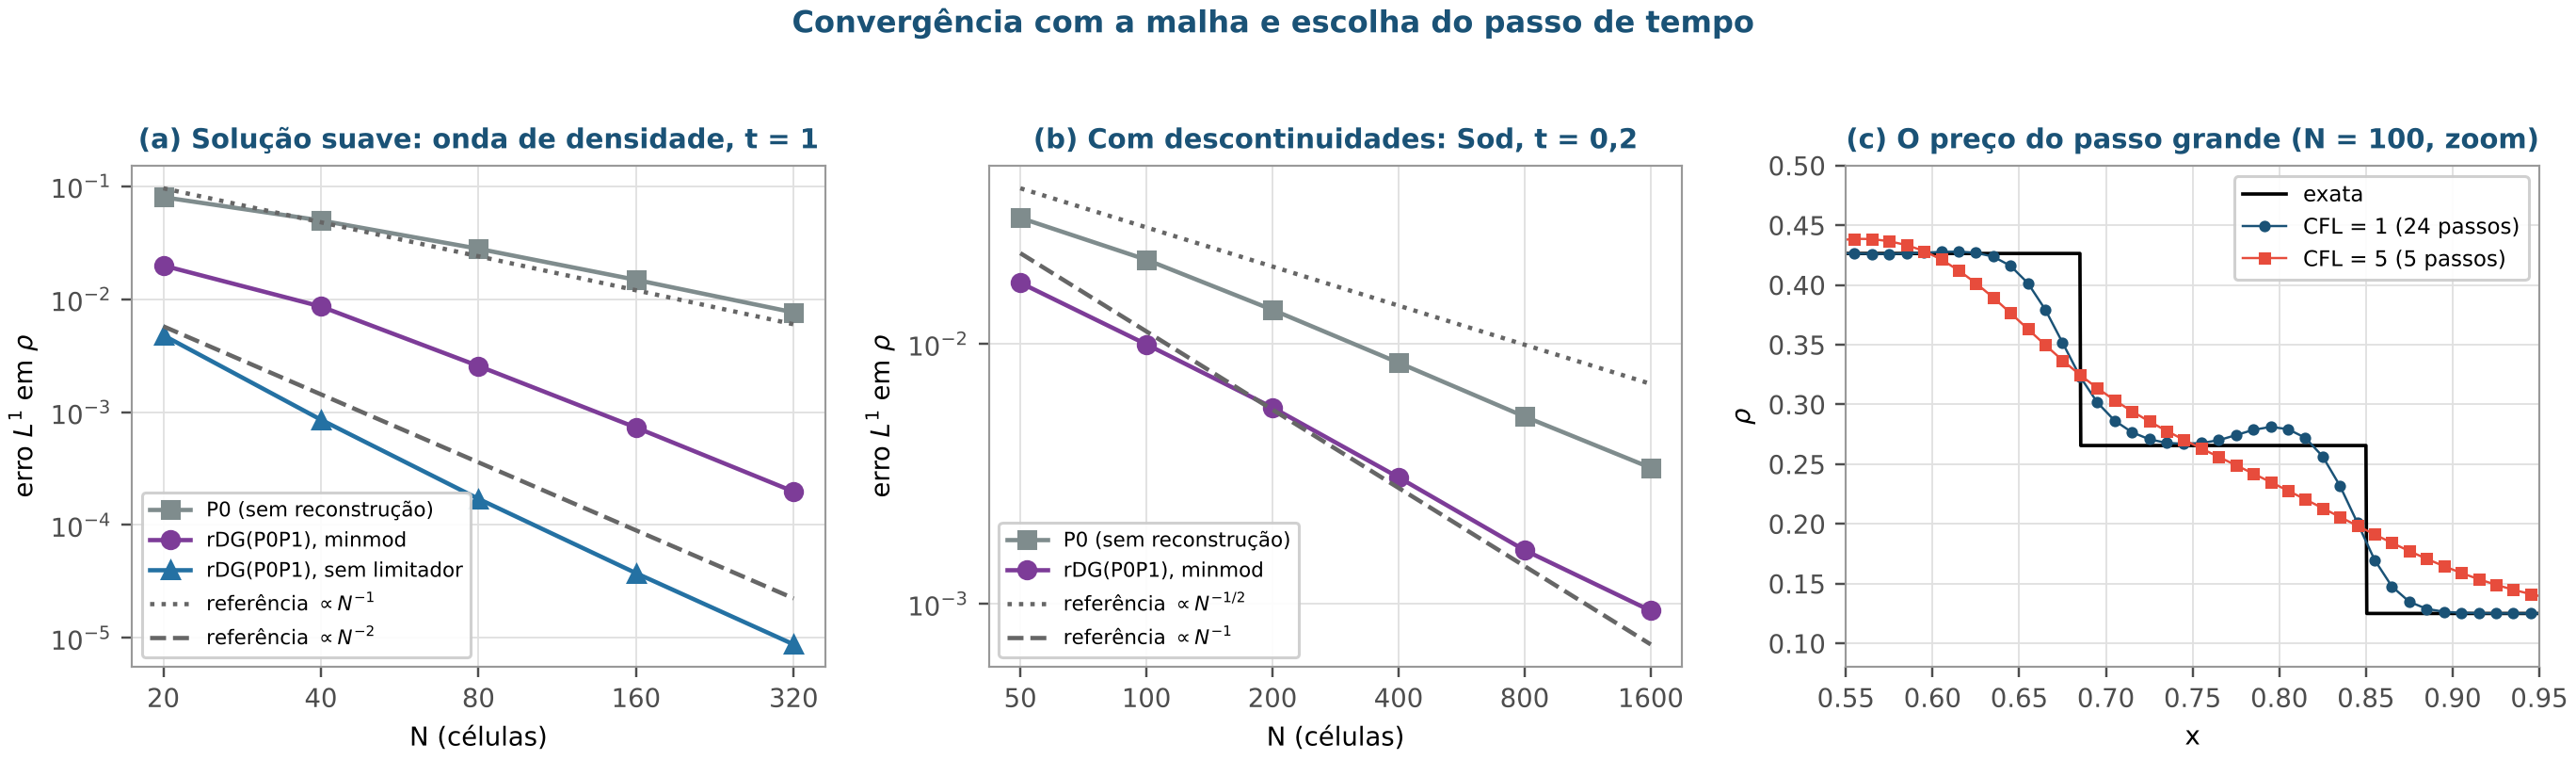
\includegraphics[width=\textwidth]{figs/fig7_convergencia.png}
\caption{Convergência com a malha e efeito do passo de tempo. (a) Onda de densidade suave: P0 segue a referência de primeira ordem, o rDG(P0P1) com minmod aproxima-se da segunda ordem e sem limitador a atinge. (b) Tubo de Sod: as descontinuidades reduzem a ordem observada dos dois métodos, mas a reconstrução mantém o erro cerca de três vezes menor. (c) O mesmo problema com $N=100$ e dois passos de tempo: com $\mathrm{CFL}=5$ o método continua estável, porém o contato e o choque ficam espalhados por muito mais células. Estabilidade incondicional não é precisão incondicional.}
\label{fig:convergencia}
\end{figure}

% ================================================================ 10
\section{Resumo e perspectivas}

\subsection{O que aprendemos}
\begin{enumerate}[leftmargin=2.5em,itemsep=3pt]
\item \textbf{Leis de conservação} descrevem o transporte de quantidades físicas; o \textbf{fluxo} $f(u)$ mede quanto passa por cada ponto. A forma integral continua válida nos choques; é dela que o método parte.
\item \textbf{Volumes finitos} discretizam a forma integral: a média celular muda conforme os fluxos nas interfaces. O que sai de uma célula entra na vizinha, logo o método é conservativo e os choques andam na velocidade certa.
\item \textbf{rDG(P0P1)} ganha segunda ordem ao reconstruir uma reta (P1) a partir das médias (P0), em vez de evoluir incógnitas adicionais como no DG puro. O coeficiente $\uh_i$ é a variação do centro até a face.
\item O \textbf{minmod} limita as inclinações para evitar oscilações, degenerando para P0 perto de descontinuidades. É um esquema TVD: nenhum extremo novo é criado.
\item O \textbf{HLLC} resolve os problemas de Riemann locais nas interfaces, capturando corretamente choques, rarefações e descontinuidades de contato. O fluxo é o da região do diagrama de ondas em que a interface cai.
\item O \textbf{BDF2} integra no tempo de forma implícita e A-estável, permitindo passos de tempo muito maiores que métodos explícitos e viabilizando a simulação de problemas com escalas de tempo díspares. O sistema não linear de cada passo pede um Newton de verdade (JFNK); o passo grande é estável, mas borra as ondas rápidas.
\end{enumerate}

\subsection{Para onde ir}

O framework rDG admite extensões naturais:
\begin{itemize}[leftmargin=2.5em,itemsep=3pt]
\item \textbf{rDG(P0P2)}: reconstrução quadrática $\to$ terceira ordem;
\item \textbf{rDG(P1P2)}: evolui $\ub$ e $\uh$ via DG, reconstrói o termo quadrático;
\item \textbf{2D/3D}: a formulação DG se adapta naturalmente a triângulos/tetraedros;
\item Limitadores mais sofisticados (WENO, Barth-Jespersen) e Riemann solvers (HLLC com correções entrópicas, Roe);
\item Reconstrução nas variáveis primitivas ou características, que deixa o contato mais nítido; limitadores que garantem positividade de $\rho$ e $p$, indispensáveis em escoamentos com vácuo ou com fases evanescentes;
\item Integradores implícitos--explícitos (IMEX), que tratam implicitamente só a parte acústica e mantêm a convecção explícita, combinando o passo grande do BDF2 com a nitidez do explícito.
\end{itemize}

\vfill
\begin{center}\small\color{cinzatexto}
Documento gerado automaticamente com \LaTeX{} e Python (NumPy + SciPy + Matplotlib).\\
Código-fonte completo disponível como material complementar: \texttt{scripts/rdg\_p0p1.py} e \texttt{scripts/make\_figs.sh}.
\end{center}

\end{document}
